\documentclass[11pt,letterpaper]{article}
\usepackage[margin=1in]{geometry}
\usepackage[T1]{fontenc}
\usepackage{lmodern,graphicx,booktabs,longtable,array,tabularx,enumitem,xcolor,hyperref,fancyhdr,float,pdflscape,tikz}
\graphicspath{{assets/}{./}}
\hypersetup{colorlinks=true,linkcolor=black,urlcolor=blue,citecolor=black}
\setlength{\parindent}{0pt}\setlength{\parskip}{6pt}
\setlength{\LTpre}{6pt}\setlength{\LTpost}{6pt}\setlength{\tabcolsep}{4pt}
\setlist{nosep}\setlength{\headheight}{14pt}
\pagestyle{fancy}\fancyhf{}\fancyhead[L]{SYSEN 5151 | StockLens}\fancyhead[R]{Function Architecture}\fancyfoot[C]{\thepage}
\emergencystretch=2em
\begin{document}
\begin{titlepage}\centering\vspace*{.75in}
{\large Cornell University\\SYSEN 5151: Foundations of Systems Engineering\par}
\vspace{.6in}{\Huge\bfseries StockLens\par}\vspace{.25in}
{\LARGE Architecture Definition: Function\par}\vspace{.2in}
{\Large Integrated Report --- Chapters 6--7\par}\vspace{.65in}
{\large Group 29\par}\vspace{.2in}
Yihan Zhou\\Shuxuan Wang\\Henian Li\\Xinyuan Yan\\David Limmer\\Rosa Szurgot
\vfill Due: October 25, 2026, 11:59 PM\\Model and report revision: October 22, 2026
\end{titlepage}
\tableofcontents\newpage
\section{Introduction}
\subsection{Purpose and Scope}
This report defines the function architecture of StockLens and evaluates whether its structure supports UC.1, \textit{Compare Stocks \& Evaluate Ranking}. It combines the Chapter 6 direct-trace method with the Chapter 7 first-level decomposition. The deliverables include the Innoslate model, a three-level function hierarchy, inherited and internal IDEF0 interfaces, a function N-squared diagram, functional requirements and a numbered scenario trace. The report presents both model contents and the reasoning behind their organization, following the assignment rubric and Lab Manual Sections 6.2.1, 6.3--6.4 and 7.2--7.4\cite{assignment,manual}.

\subsection{Evidence and Method}
The authoritative model is Innoslate project 659, \textit{AI-Assisted Stock Platform}. The context metafunction is MF.0 (264781); the system-of-interest function is F.0 \textit{Provide Stock Comparisons} (264782). The team-supplied final requirements report is the upstream baseline\cite{baseline}. Existing system requirement numbers and entities are retained. The model revision first established the missing first-level functions, carried down every inherited ICOM, added internal flows, decomposed the hierarchy to three levels, and then reconciled the use-case messages and requirements allocations.

Native diagram exports are reproduced as evidence. Where native boxes abbreviate names, the adjacent tables provide the complete names and IDs. The PowerPoint trace adds editable color and number annotations to the native first-level export. A separate function-level sequence explicitly displays internal flows that are abstracted inside the StockLens lifeline of the native actor sequence. Gray exchanges 0 and 9 are now drawn explicitly as configuration and maintainer-status messages, so every numbered IDEF0 exchange has a visible sequence counterpart. Recorded structural checks support model consistency; they do not establish live-provider performance or stakeholder acceptance.

\section{Function Architecture}
\subsection{Boundary, Concerns and Architecture Drivers}
StockLens is a research decision-support system. It accepts two eligible stock symbols and a common analysis date, calculates comparable scores, explains their computed drivers, and presents inspectable sources and dates. Research User, Market Data Provider, News Provider, AI Model Service and System Maintainer are external participants. StockLens owns request validation, evidence orchestration, deterministic ranking, explanation coordination and presentation. Automated trading, order execution, personalized portfolios and intraday support are excluded.

The final requirements baseline fixes ten candidate symbols, a common cutoff and 21 aligned adjusted-price observations for 20 daily returns. It uses 20-day momentum and unannualized sample volatility with equal weights and average-tie-rank normalization across the same frozen universe. News does not affect the numerical score. No missing prices are imputed and the normalization universe is not silently reduced. Score differences within $10^{-6}$ points are ties; display uses two decimal places\cite{baseline}. These are inherited educational comparison rules, not evidence that the scoring rule predicts investment returns.

Three stakeholder concerns drive the decomposition. Comparable calculations require validation before scoring. Explanations must remain tied to authoritative driver values, so external AI is separated from ranking. Inspectable evidence requires source identities and distinct analysis, observation and publication dates to survive every handoff. Research Configuration is a control on all five functions; it is not a provider response or a per-function physical mechanism. The selected architecture preserves the original system boundary and external ICOM meanings.

\subsubsection{Stakeholder Concerns and Selected Viewpoints}
The architecture-driver tags retain the upstream candidates: PNFR-01 (understandability) motivates exact computed-driver values and the F.3/F.4 separation; PNFR-02 (operability) motivates versioned configuration, explicit status and a reproducible run procedure; PNFR-03 (evidence inspectability) motivates source/date preservation from F.2 through F.5. These report-level driver tags do not promote unvalidated suitability candidates into passed functional requirements.
\begin{tabularx}{\linewidth}{@{}p{.23\linewidth}X@{}}\toprule
Viewpoint & Concern and selected representation\\\midrule
Boundary and responsibility & Context IDEF0 identifies StockLens, its five external participant functions and performing mechanisms.\\
Functional structure & Three-level hierarchy and readable branch views separate validation, evidence, calculation, explanation and presentation.\\
Behavior and continuity & Action/sequence views and the numbered IDEF0 trace show one complete comparison scenario, including control/status context.\\
Internal interfaces & N-squared matrix and contract v1 show each source, destination and machine-readable handoff.\\
Requirement assurance & The sixteen-row requirement table links obligations, rationale, MOPs, verification criteria and responsible functions.\\\bottomrule\end{tabularx}

The current physical allocation remains F.0 to StockLens and one mechanism per external context function. First-level physical alternatives and subsystem allocation are staged after this functional lesson, consistent with the explicit mechanism deferral in Section 7.2.2; the functional decomposition does not silently allocate every child to a prematurely selected component.

\subsection{Functional Elements and Three-Level Hierarchy}
The hierarchy is rooted at F.0, followed by five first-level functions and ten next-level functions. The first level separates responsibilities rather than external participants. Each branch contains two lower-level functions. This gives an overall view of organization while allowing the lower-level names and boundaries to be explained without crowding a single diagram.
\begin{figure}[H]\centering
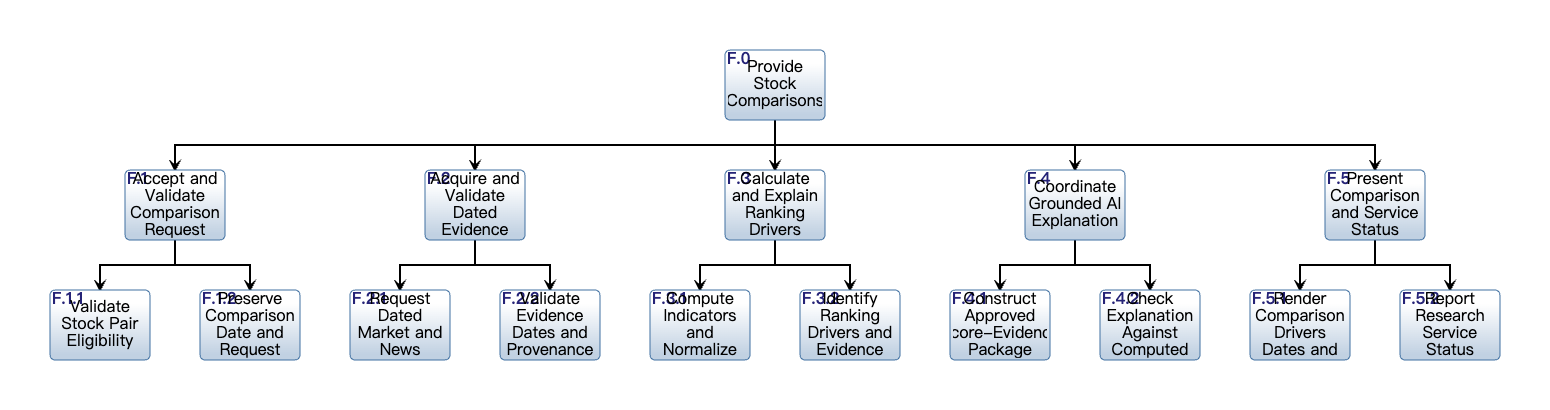
\includegraphics[width=\linewidth,height=.78\textheight,keepaspectratio]{hierarchy-overview.png}
\caption{Native Innoslate three-level function hierarchy rooted at F.0 (264782).}\label{fig:hierarchy}\end{figure}
{\small
\begin{longtable}{@{}>{\raggedright\arraybackslash}p{0.13\linewidth}>{\raggedright\arraybackslash}p{0.26\linewidth}>{\raggedright\arraybackslash}p{0.55\linewidth}@{}}
\caption{First-level functions and their complete definitions.}\\
\toprule ID / entity & Function & Responsibility and boundary\\\midrule\endfirsthead
\toprule ID / entity & Function & Responsibility and boundary\\\midrule\endhead
F.1 / 269034 & Accept and Validate Comparison Request & Accept the two stock symbols and common analysis date under the maintained research configuration. Validate eligibility and request completeness, then supply a validated comparison request to evidence acquisition. Preserve the request identity and date through the downstream calculation. This is a functional decomposition of F.0, not an allocation to a physical subsystem.\\[5pt]
F.2 / 269035 & Acquire and Validate Dated Evidence & Acquire dated market records and attributable news evidence for the validated stock pair and common analysis date. Issue distinct market and news queries, check symbol/date coverage and required provenance fields, and send validated evidence to ranking. Preserve observation and publication dates separately from the analysis date.\\[5pt]
F.3 / 269036 & Calculate and Explain Ranking Drivers & Calculate deterministic indicator values and normalized ranking scores from validated dated evidence under the recorded scoring configuration. Identify computed drivers and retain their exact values. Produce a score-and-driver record for explanation coordination and direct display; external AI wording must not alter scores or ordering.\\[5pt]
F.4 / 269037 & Coordinate Grounded AI Explanation & Construct the approved score-evidence package from already computed scores, driver values and dated sources, send it to the external AI Model Service, and validate the returned explanation against those values and sources. Preserve deterministic ranking when the explanation is unavailable or fails validation.\\[5pt]
F.5 / 269038 & Present Comparison and Service Status & Assemble and present the comparison using authoritative calculated scores, indicator drivers, source links and distinct analysis/observation/publication dates. Include a checked explanation or an explicit unavailable state without changing calculated ranking. Expose the supporting evidence for the research user to inspect and provide service status to the maintainer.\\[5pt]
\bottomrule\end{longtable}
}
\subsubsection{Readable Branch Views}
\begin{figure}[H]\centering
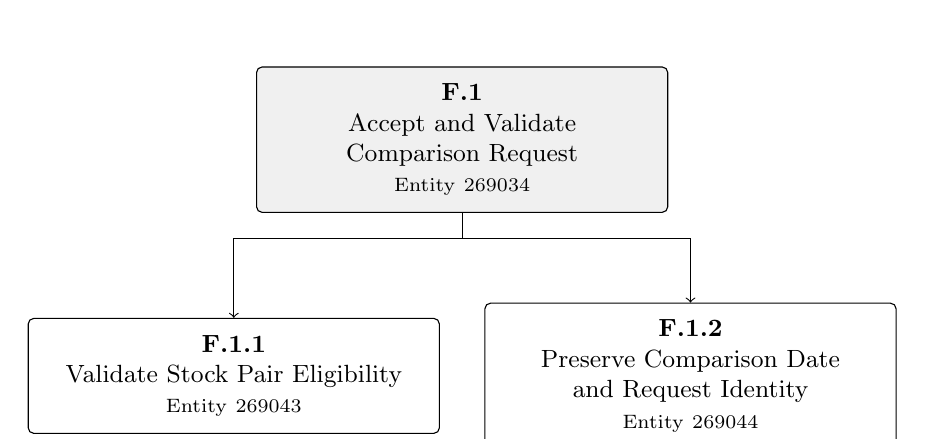
\begin{tikzpicture}[nodebox/.style={draw,rounded corners=2pt,align=center,text width=4.8cm,minimum height=1.4cm,font=\small,inner sep=6pt}]
\node[nodebox,fill=gray!12] (p) at (0,0) {\textbf{F.1}\\Accept and Validate Comparison Request\\{\scriptsize Entity 269034}};
\node[nodebox] (c0) at (-2.9,-3) {\textbf{F.1.1}\\Validate Stock Pair Eligibility\\{\scriptsize Entity 269043}};
\draw[->] (p.south) -- (0,-1.25) -| (c0.north);
\node[nodebox] (c1) at (2.9,-3) {\textbf{F.1.2}\\Preserve Comparison Date and Request Identity\\{\scriptsize Entity 269044}};
\draw[->] (p.south) -- (0,-1.25) -| (c1.north);
\end{tikzpicture}
\caption{Readable projection of the saved native branch for F.1 Accept and Validate Comparison Request.}\label{fig:branch1}\end{figure}
\begin{longtable}{@{}>{\raggedright\arraybackslash}p{0.35\linewidth}>{\raggedright\arraybackslash}p{0.6\linewidth}@{}}
\caption{Definitions for the F.1 branch.}\\
\toprule Lower-level function & Definition\\\midrule\endfirsthead
\toprule Lower-level function & Definition\\\midrule\endhead
F.1.1 Validate Stock Pair Eligibility & Check that both supplied symbols belong to the configured eligible stock universe and that the pair identifies the requested comparison.\\[5pt]
F.1.2 Preserve Comparison Date and Request Identity & Normalize the common analysis date and associate it with the selected pair and request identifier so downstream results remain attributable to the original request.\\[5pt]
\bottomrule\end{longtable}
\begin{figure}[H]\centering
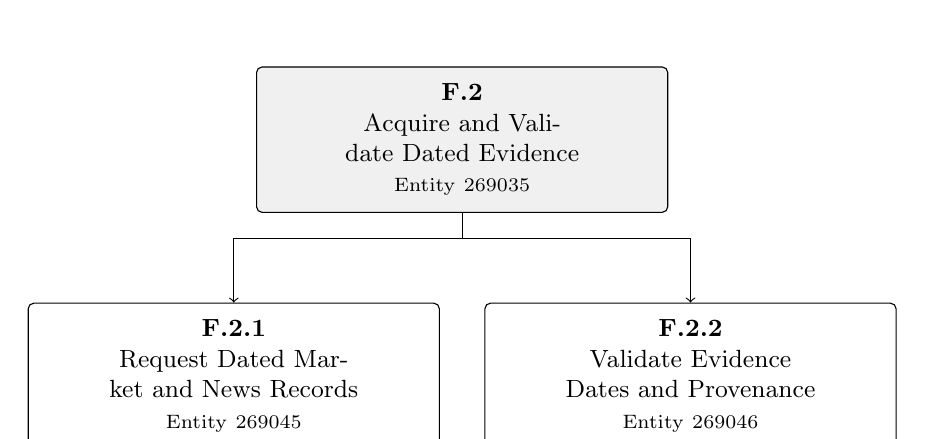
\begin{tikzpicture}[nodebox/.style={draw,rounded corners=2pt,align=center,text width=4.8cm,minimum height=1.4cm,font=\small,inner sep=6pt}]
\node[nodebox,fill=gray!12] (p) at (0,0) {\textbf{F.2}\\Acquire and Validate Dated Evidence\\{\scriptsize Entity 269035}};
\node[nodebox] (c0) at (-2.9,-3) {\textbf{F.2.1}\\Request Dated Market and News Records\\{\scriptsize Entity 269045}};
\draw[->] (p.south) -- (0,-1.25) -| (c0.north);
\node[nodebox] (c1) at (2.9,-3) {\textbf{F.2.2}\\Validate Evidence Dates and Provenance\\{\scriptsize Entity 269046}};
\draw[->] (p.south) -- (0,-1.25) -| (c1.north);
\end{tikzpicture}
\caption{Readable projection of the saved native branch for F.2 Acquire and Validate Dated Evidence.}\label{fig:branch2}\end{figure}
\begin{longtable}{@{}>{\raggedright\arraybackslash}p{0.35\linewidth}>{\raggedright\arraybackslash}p{0.6\linewidth}@{}}
\caption{Definitions for the F.2 branch.}\\
\toprule Lower-level function & Definition\\\midrule\endfirsthead
\toprule Lower-level function & Definition\\\midrule\endhead
F.2.1 Request Dated Market and News Records & Issue separately addressed market and news queries for the validated symbols and analysis context. Preserve each provider request and response association.\\[5pt]
F.2.2 Validate Evidence Dates and Provenance & Check symbol coverage, required observations, source identifiers and publication dates; retain distinct analysis, observation and publication dates in the validated evidence record.\\[5pt]
\bottomrule\end{longtable}
\begin{figure}[H]\centering
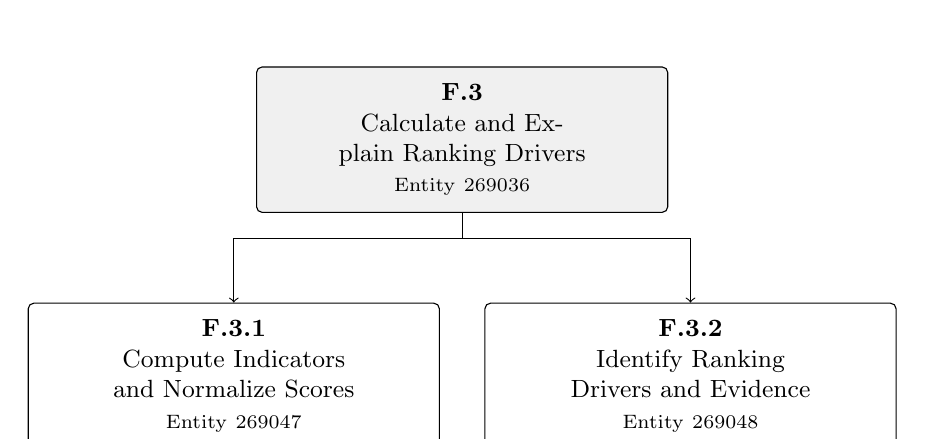
\begin{tikzpicture}[nodebox/.style={draw,rounded corners=2pt,align=center,text width=4.8cm,minimum height=1.4cm,font=\small,inner sep=6pt}]
\node[nodebox,fill=gray!12] (p) at (0,0) {\textbf{F.3}\\Calculate and Explain Ranking Drivers\\{\scriptsize Entity 269036}};
\node[nodebox] (c0) at (-2.9,-3) {\textbf{F.3.1}\\Compute Indicators and Normalize Scores\\{\scriptsize Entity 269047}};
\draw[->] (p.south) -- (0,-1.25) -| (c0.north);
\node[nodebox] (c1) at (2.9,-3) {\textbf{F.3.2}\\Identify Ranking Drivers and Evidence\\{\scriptsize Entity 269048}};
\draw[->] (p.south) -- (0,-1.25) -| (c1.north);
\end{tikzpicture}
\caption{Readable projection of the saved native branch for F.3 Calculate and Explain Ranking Drivers.}\label{fig:branch3}\end{figure}
\begin{longtable}{@{}>{\raggedright\arraybackslash}p{0.35\linewidth}>{\raggedright\arraybackslash}p{0.6\linewidth}@{}}
\caption{Definitions for the F.3 branch.}\\
\toprule Lower-level function & Definition\\\midrule\endfirsthead
\toprule Lower-level function & Definition\\\midrule\endhead
F.3.1 Compute Indicators and Normalize Scores & Calculate the documented indicators and normalized weighted comparison scores from the validated records using one configuration for both stocks.\\[5pt]
F.3.2 Identify Ranking Drivers and Evidence & Select computed ranking drivers and their exact values and retain supporting dated sources without allowing generated narrative to alter calculated scores.\\[5pt]
\bottomrule\end{longtable}
\begin{figure}[H]\centering
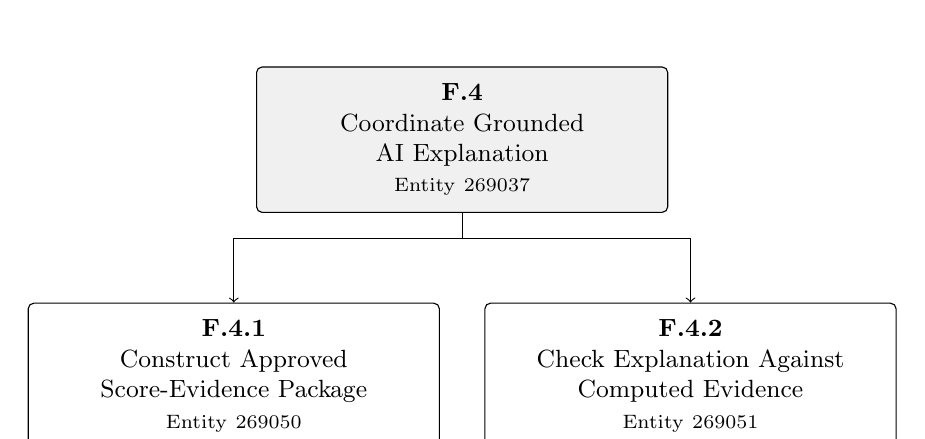
\begin{tikzpicture}[nodebox/.style={draw,rounded corners=2pt,align=center,text width=4.8cm,minimum height=1.4cm,font=\small,inner sep=6pt}]
\node[nodebox,fill=gray!12] (p) at (0,0) {\textbf{F.4}\\Coordinate Grounded AI Explanation\\{\scriptsize Entity 269037}};
\node[nodebox] (c0) at (-2.9,-3) {\textbf{F.4.1}\\Construct Approved Score-Evidence Package\\{\scriptsize Entity 269050}};
\draw[->] (p.south) -- (0,-1.25) -| (c0.north);
\node[nodebox] (c1) at (2.9,-3) {\textbf{F.4.2}\\Check Explanation Against Computed Evidence\\{\scriptsize Entity 269051}};
\draw[->] (p.south) -- (0,-1.25) -| (c1.north);
\end{tikzpicture}
\caption{Readable projection of the saved native branch for F.4 Coordinate Grounded AI Explanation.}\label{fig:branch4}\end{figure}
\begin{longtable}{@{}>{\raggedright\arraybackslash}p{0.35\linewidth}>{\raggedright\arraybackslash}p{0.6\linewidth}@{}}
\caption{Definitions for the F.4 branch.}\\
\toprule Lower-level function & Definition\\\midrule\endfirsthead
\toprule Lower-level function & Definition\\\midrule\endhead
F.4.1 Construct Approved Score-Evidence Package & Prepare the external AI request using computed scores, selected driver values, source identifiers and date context under the approved field schema.\\[5pt]
F.4.2 Check Explanation Against Computed Evidence & Compare the returned narrative with authoritative driver values and sources; expose a checked explanation or an unavailable state while preserving calculated ranking.\\[5pt]
\bottomrule\end{longtable}
\begin{figure}[H]\centering
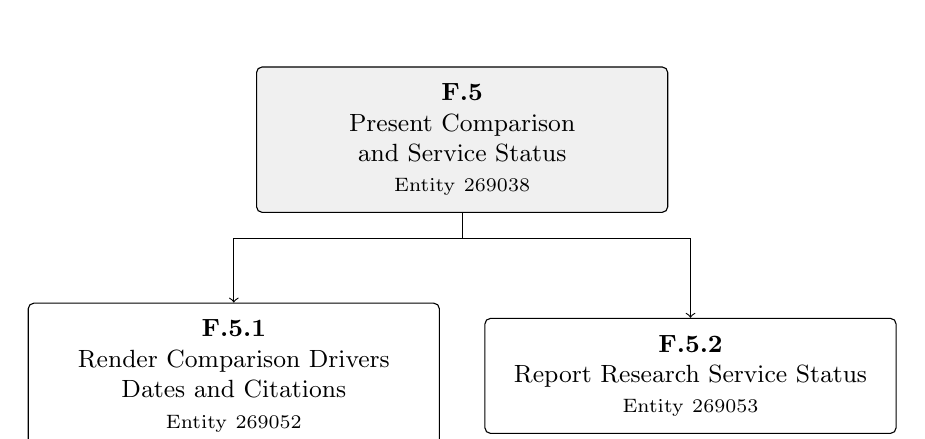
\begin{tikzpicture}[nodebox/.style={draw,rounded corners=2pt,align=center,text width=4.8cm,minimum height=1.4cm,font=\small,inner sep=6pt}]
\node[nodebox,fill=gray!12] (p) at (0,0) {\textbf{F.5}\\Present Comparison and Service Status\\{\scriptsize Entity 269038}};
\node[nodebox] (c0) at (-2.9,-3) {\textbf{F.5.1}\\Render Comparison Drivers Dates and Citations\\{\scriptsize Entity 269052}};
\draw[->] (p.south) -- (0,-1.25) -| (c0.north);
\node[nodebox] (c1) at (2.9,-3) {\textbf{F.5.2}\\Report Research Service Status\\{\scriptsize Entity 269053}};
\draw[->] (p.south) -- (0,-1.25) -| (c1.north);
\end{tikzpicture}
\caption{Readable projection of the saved native branch for F.5 Present Comparison and Service Status.}\label{fig:branch5}\end{figure}
\begin{longtable}{@{}>{\raggedright\arraybackslash}p{0.35\linewidth}>{\raggedright\arraybackslash}p{0.6\linewidth}@{}}
\caption{Definitions for the F.5 branch.}\\
\toprule Lower-level function & Definition\\\midrule\endfirsthead
\toprule Lower-level function & Definition\\\midrule\endhead
F.5.1 Render Comparison Drivers Dates and Citations & Display the deterministic comparison, exact driver values, supporting source links, distinct dates, and the checked explanation or explicit unavailable state for user inspection.\\[5pt]
F.5.2 Report Research Service Status & Provide maintainer-visible status for the configured comparison workflow, including explanation availability, without representing incomplete service evidence as successful validation.\\[5pt]
\bottomrule\end{longtable}

\subsection{Top-Level and First-Level IDEF0}
The context diagram places F.0 alongside five external functions. Each context function retains its existing performing mechanism. Decomposing F.0 creates the five internal functions; external participant functions are not relabeled as internal work. The first-level IDEF0 carries down four inputs, one control and five outputs from F.0. It adds four distinct internal I/O entities, with five directed internal connections because IF.03 fans out to both explanation coordination and presentation.
\begin{figure}[H]\centering
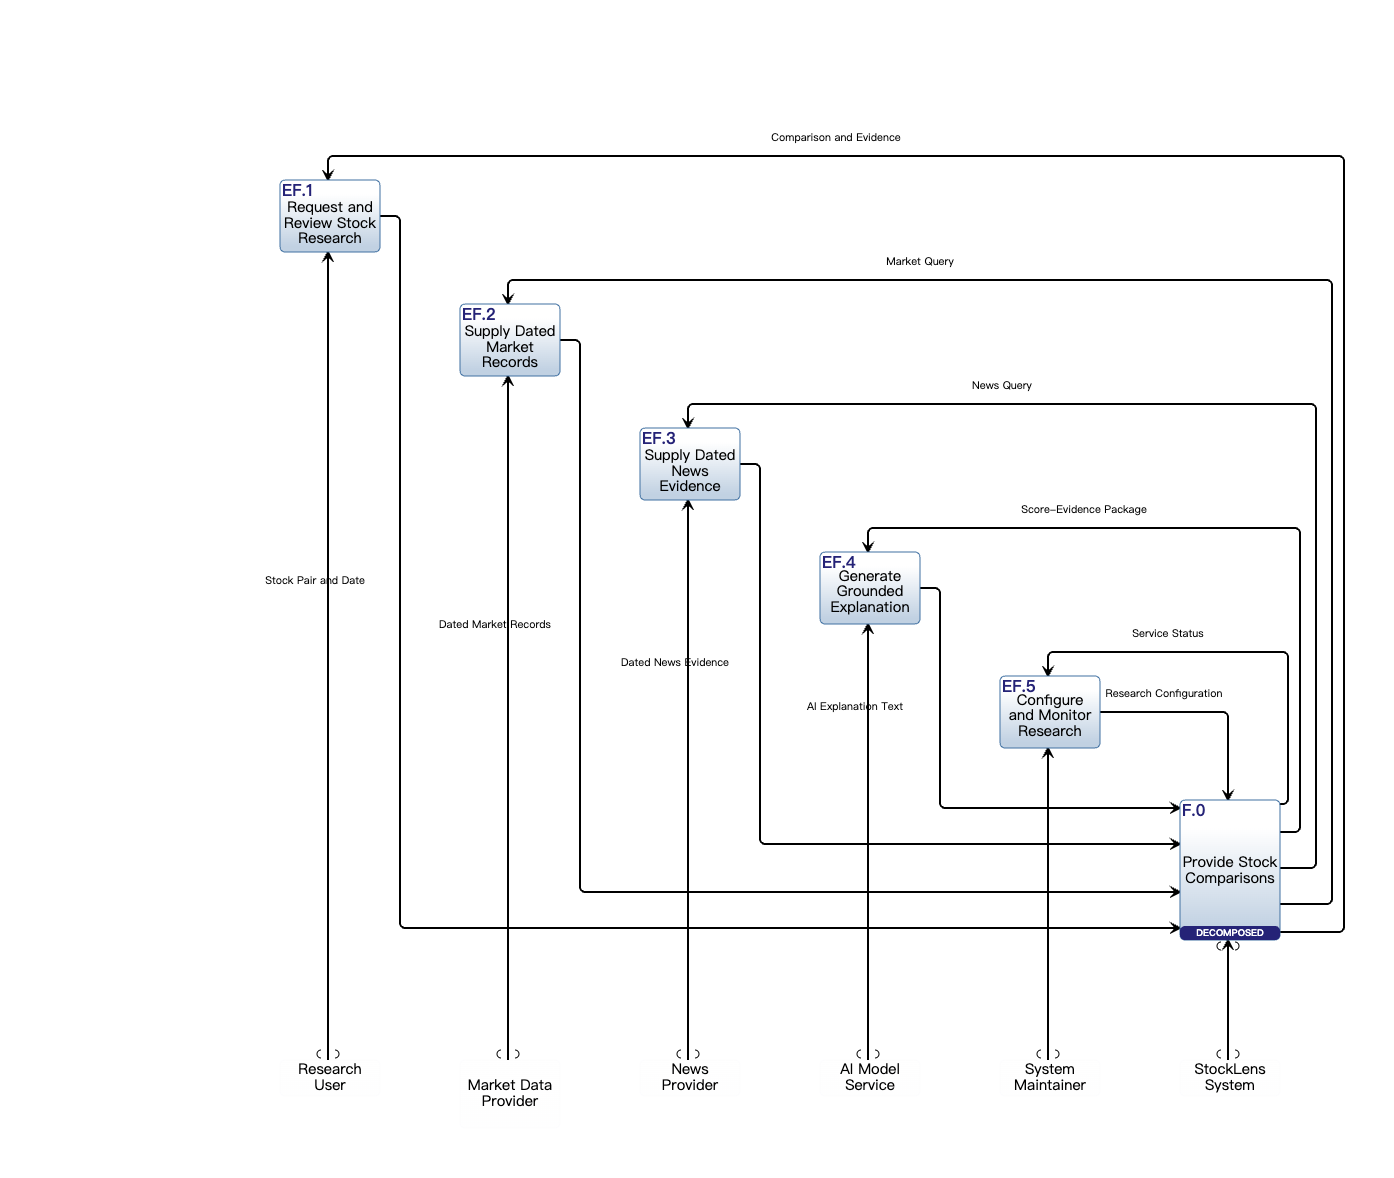
\includegraphics[width=\linewidth,height=.78\textheight,keepaspectratio]{idef0-top-level.png}
\caption{Native MF.0 context IDEF0; system and external functions retain their original boundary roles.}\label{fig:context}\end{figure}
\begin{figure}[H]\centering
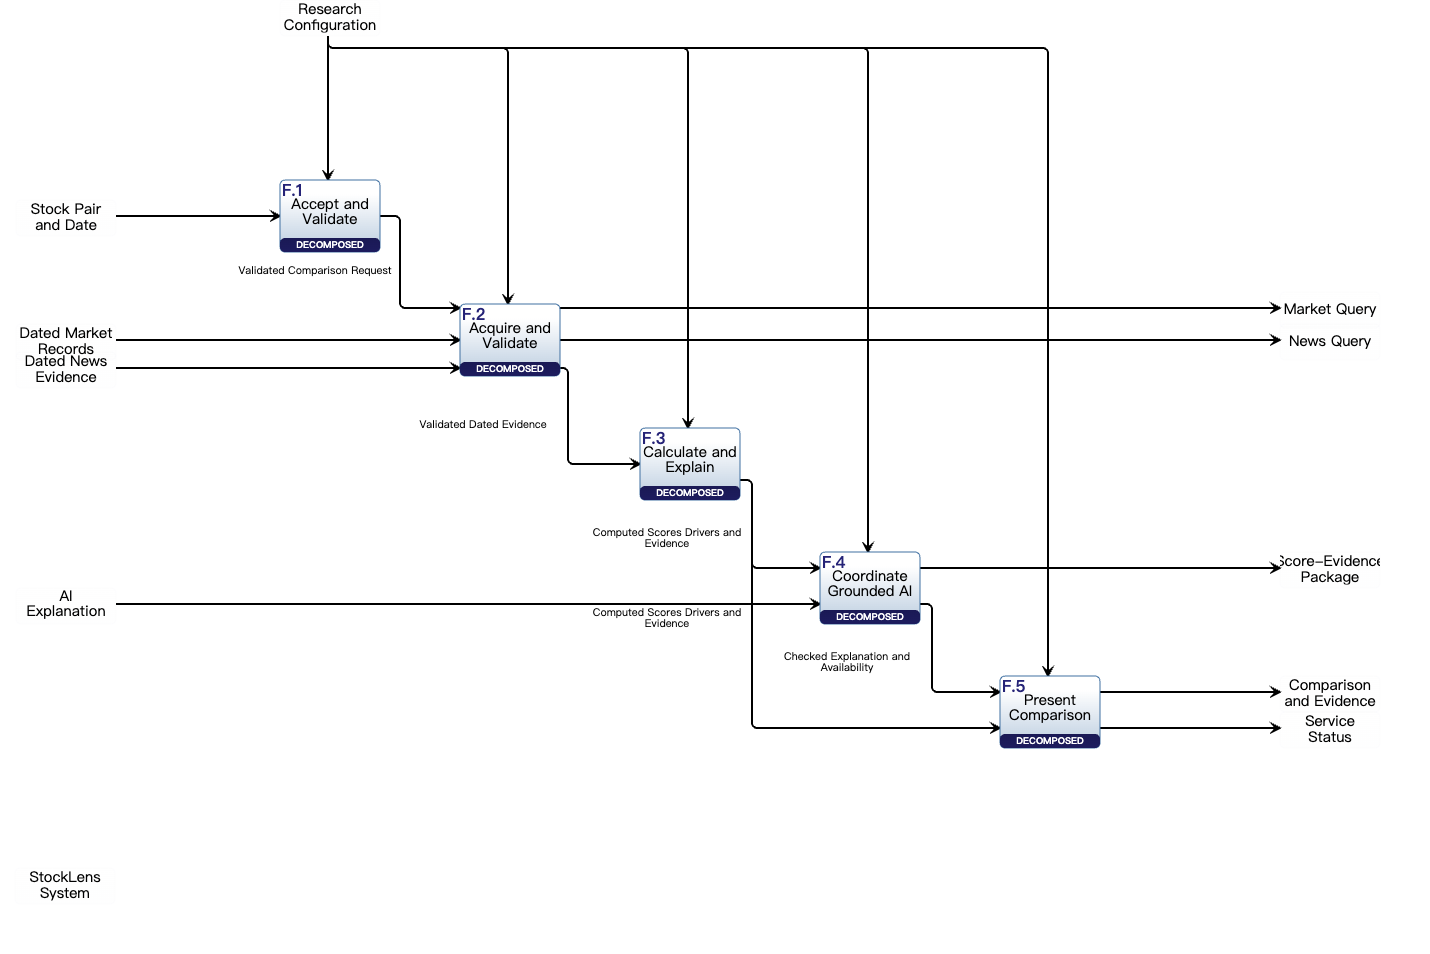
\includegraphics[width=\linewidth,height=.78\textheight,keepaspectratio]{idef0-first-level.png}
\caption{Native F.0 first-level IDEF0 after interface allocation to the lower-level functions.}\label{fig:first}\end{figure}
{\small
\begin{longtable}{@{}>{\raggedright\arraybackslash}p{0.09\linewidth}>{\raggedright\arraybackslash}p{0.1\linewidth}>{\raggedright\arraybackslash}p{0.3\linewidth}>{\raggedright\arraybackslash}p{0.45\linewidth}@{}}
\caption{Complete inherited ICOM allocation; existing interface entities are reused.}\\
\toprule Entity & ICOM & Exchange & First-level allocation\\\midrule\endfirsthead
\toprule Entity & ICOM & Exchange & First-level allocation\\\midrule\endhead
IO.01 & Input & Stock Pair and Date & Research User $\rightarrow$ F.1\\[5pt]
IO.07 & Input & Dated Market Records & Market Data Provider $\rightarrow$ F.2\\[5pt]
IO.08 & Input & Dated News Evidence & News Provider $\rightarrow$ F.2\\[5pt]
IO.09 & Input & AI Explanation Text & AI Model Service $\rightarrow$ F.4\\[5pt]
IO.10 & Control & Research Configuration & System Maintainer $\rightarrow$ F.1--F.5\\[5pt]
IO.02 & Output & Comparison and Evidence & F.5 $\rightarrow$ Research User\\[5pt]
IO.03 & Output & Market Query & F.2 $\rightarrow$ Market Data Provider\\[5pt]
IO.04 & Output & News Query & F.2 $\rightarrow$ News Provider\\[5pt]
IO.05 & Output & Score-Evidence Package & F.4 $\rightarrow$ AI Model Service\\[5pt]
IO.06 & Output & Service Status & F.5 $\rightarrow$ System Maintainer\\[5pt]
\bottomrule\end{longtable}
}

Inputs supply the selected request, dated observations, dated evidence and explanatory text. Outputs request external records, send already computed evidence for explanation, deliver the coherent comparison, and expose operational status. Research Configuration governs eligibility, the common comparison basis, allowed analysis content and status interpretation. Mechanisms remain unallocated at the first level, as required by the Lab Manual; the existing system mechanism is not replicated across the five child functions.

The lower-level allocations were checked in both directions: every first-level received flow is received by at least one child, and every first-level generated flow is generated by at least one child. Lower-level LF.01--LF.05 connect the two functions in each branch. This removes the I/O tunnels introduced when the hierarchy was expanded. It does not require physical subsystem allocation at this stage.

\subsection{Internal Interfaces and N-Squared Analysis}
\begin{table}[H]\centering\small
\begin{tabular}{@{}lccccc@{}}\toprule Source / destination & F.1 & F.2 & F.3 & F.4 & F.5\\\midrule
F.1 & --- & IF.01 & & & \\
F.2 & & --- & IF.02 & & \\
F.3 & & & --- & IF.03 & IF.03\\
F.4 & & & & --- & IF.04\\
F.5 & & & & & ---\\\bottomrule\end{tabular}
\caption{Readable N-squared cross-check. Five populated off-diagonal cells represent four distinct internal I/O entities. Empty cells do not imply a hidden connection.}\end{table}

\begin{longtable}{@{}>{\raggedright\arraybackslash}p{0.09\linewidth}>{\raggedright\arraybackslash}p{0.27\linewidth}>{\raggedright\arraybackslash}p{0.23\linewidth}>{\raggedright\arraybackslash}p{0.35\linewidth}@{}}
\caption{First-level internal interfaces from the saved model.}\\
\toprule ID & Internal exchange & Direction & Purpose\\\midrule\endfirsthead
\toprule ID & Internal exchange & Direction & Purpose\\\midrule\endhead
IF.01 & Validated Comparison Request & F.1 $\rightarrow$ F.2 & Eligible symbols, common date and request association.\\[5pt]
IF.02 & Validated Dated Evidence & F.2 $\rightarrow$ F.3 & Checked market/news records with provenance and distinct dates.\\[5pt]
IF.03 & Computed Scores Drivers and Evidence & F.3 $\rightarrow$ F.4; F.3 $\rightarrow$ F.5 & One authoritative computed record; the display receives the same scores supplied for explanation.\\[5pt]
IF.04 & Checked Explanation and Availability & F.4 $\rightarrow$ F.5 & Validated narrative or explicit unavailable state; numerical ranking is preserved.\\[5pt]
\bottomrule\end{longtable}
\begin{figure}[H]\centering
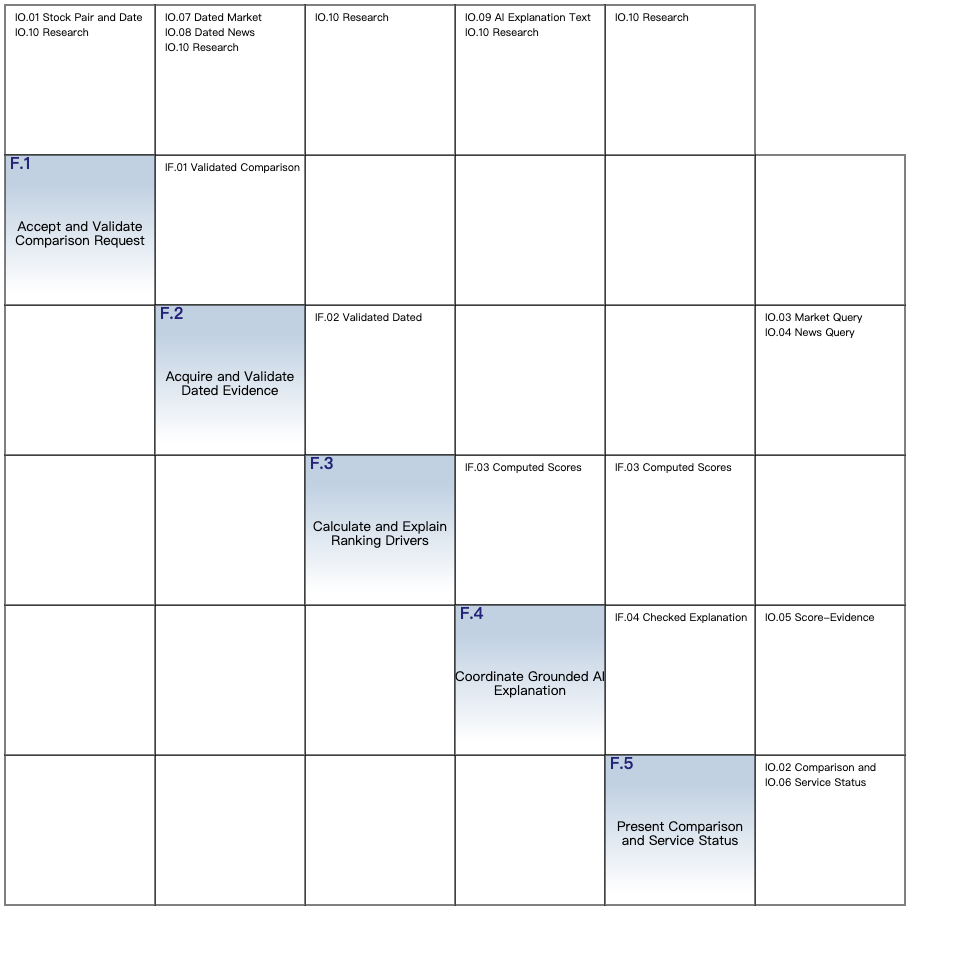
\includegraphics[width=\linewidth,height=.78\textheight,keepaspectratio]{n2-diagram.png}
\caption{Native function N-squared diagram rooted at F.0.}\label{fig:n2}\end{figure}

Read the N-squared matrix with the sending function on the row and the receiving function on the column. Functions occupy the diagonal; external inputs and controls appear on the top boundary and outputs on the right boundary. Nonempty internal cells are F.1/F.2 (IF.01), F.2/F.3 (IF.02), F.3/F.4 and F.3/F.5 (IF.03), and F.4/F.5 (IF.04). All other off-diagonal cells are empty in this first-level nominal architecture.

The IF.03 fan-out is deliberate: the presentation function receives the authoritative numerical record directly instead of reconstructing it from generated text. IF.04 supplies explanatory availability separately. The matrix therefore exposes both the calculation path and the supporting narrative path. Query/response exchanges with providers remain on the boundary, not disguised as function-to-function internal edges.

\section{Use-Case Tracing and Architecture Evaluation}
\subsection{Scenario and Corrected Native Diagrams}
UC.1 begins when the Research User selects the pair and common analysis date and ends when the user inspects the displayed drivers and citations. Dashboard/UI transports the request and renders the result; StockLens performs data coordination and calculation; the two data providers return evidence; the AI service supplies explanatory text. The selected trace covers this nominal research scenario. Maintainer configuration is its precondition, and Service Status is a separate inherited operational exchange.

The former combined UC.1.3 data request was refined into UC.1.3.1 \textit{Request Dated News Evidence} (269054) and UC.1.3.2 \textit{Request Dated Market Records} (186194). Both consume the same API Request Payload. News Fetch Command is delivered only to UC.1.4.2; Market Data Fetch Command is delivered only to UC.1.4.1. This replaces an ambiguous shared command with two independently inspectable query/return paths. The numbers follow the displayed sequence; the independent request branches may also execute concurrently.

UC.1.5 (186307) is now named \textit{Calculate Ranking and Send Computed Evidence}. Its performer remains StockLens System (171150). Its outgoing message represents the handoff after local calculation, not an instruction for AI to choose scores. UC.1.8 is explicitly documented as a terminal human inspection consuming Synchronized Visual Display. Because it produces no further message in this scenario, the native sequence ends with the dashboard-to-user exchange; the function-level sequence marks the final inspection as an endpoint note.
\begin{figure}[H]\centering
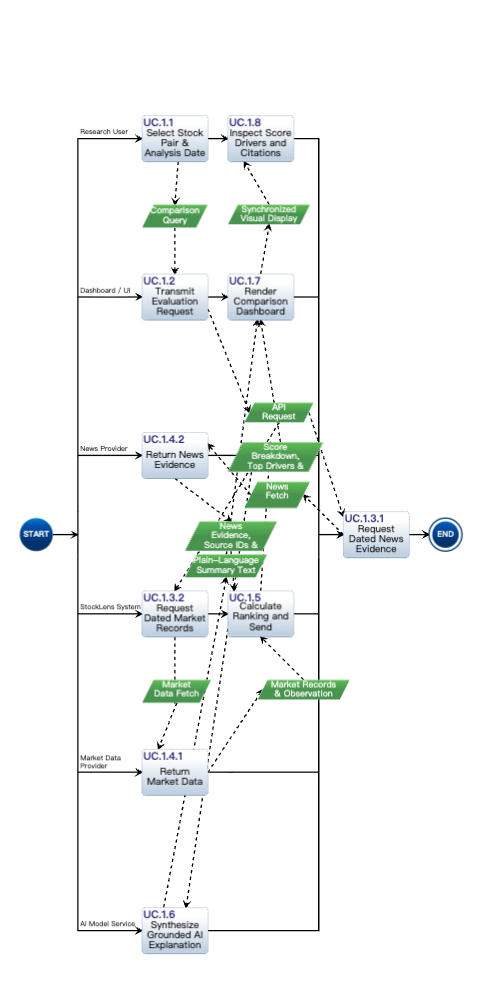
\includegraphics[width=\linewidth,height=.78\textheight,keepaspectratio]{action-diagram.png}
\caption{Updated native UC.1 action diagram with separate news and market query actions.}\label{fig:action}\end{figure}
\begin{figure}[H]\centering
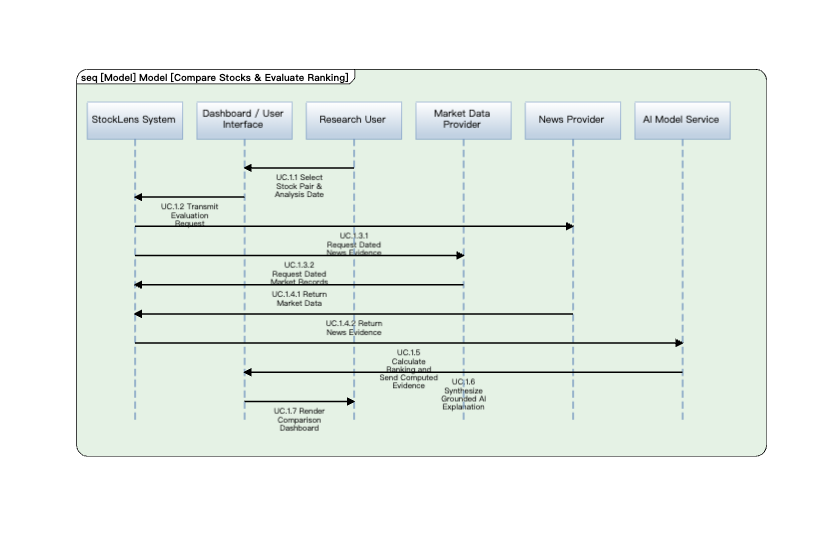
\includegraphics[width=\linewidth,height=.78\textheight,keepaspectratio]{sequence-native.png}
\caption{Updated native actor sequence. Message labels use unique UC action numbers; final inspection is a terminal observation.}\label{fig:native-seq}\end{figure}

\subsection{Direct Trace Method}
The trace follows Lab Manual Section 6.2.1. Plain numbers identify the inherited exchanges in one legal ordering of the scenario. Hierarchical subnumbers identify first-level internal flows. Step 1 is refined by 1.1; evidence acquisition is followed by 5.1--5.3; the AI return is followed by 7.1. Blue highlights inherited scenario exchanges and green highlights internal flows. Number 0 identifies the configuration precondition; gray number 9 retains the maintenance-status exchange outside the selected user path.

The native actor sequence abstracts StockLens internal functions into one lifeline. The refined sequence below makes those internal handoffs explicit at the functional abstraction, without assigning physical mechanisms. Both the refined sequence and the annotated IDEF0 use exactly the same trace numbers. Figure arrows, labels and the mapping table are intended to be checked together; a line crossing is not an implied connection.
\clearpage\begin{landscape}
\begin{figure}[H]\centering
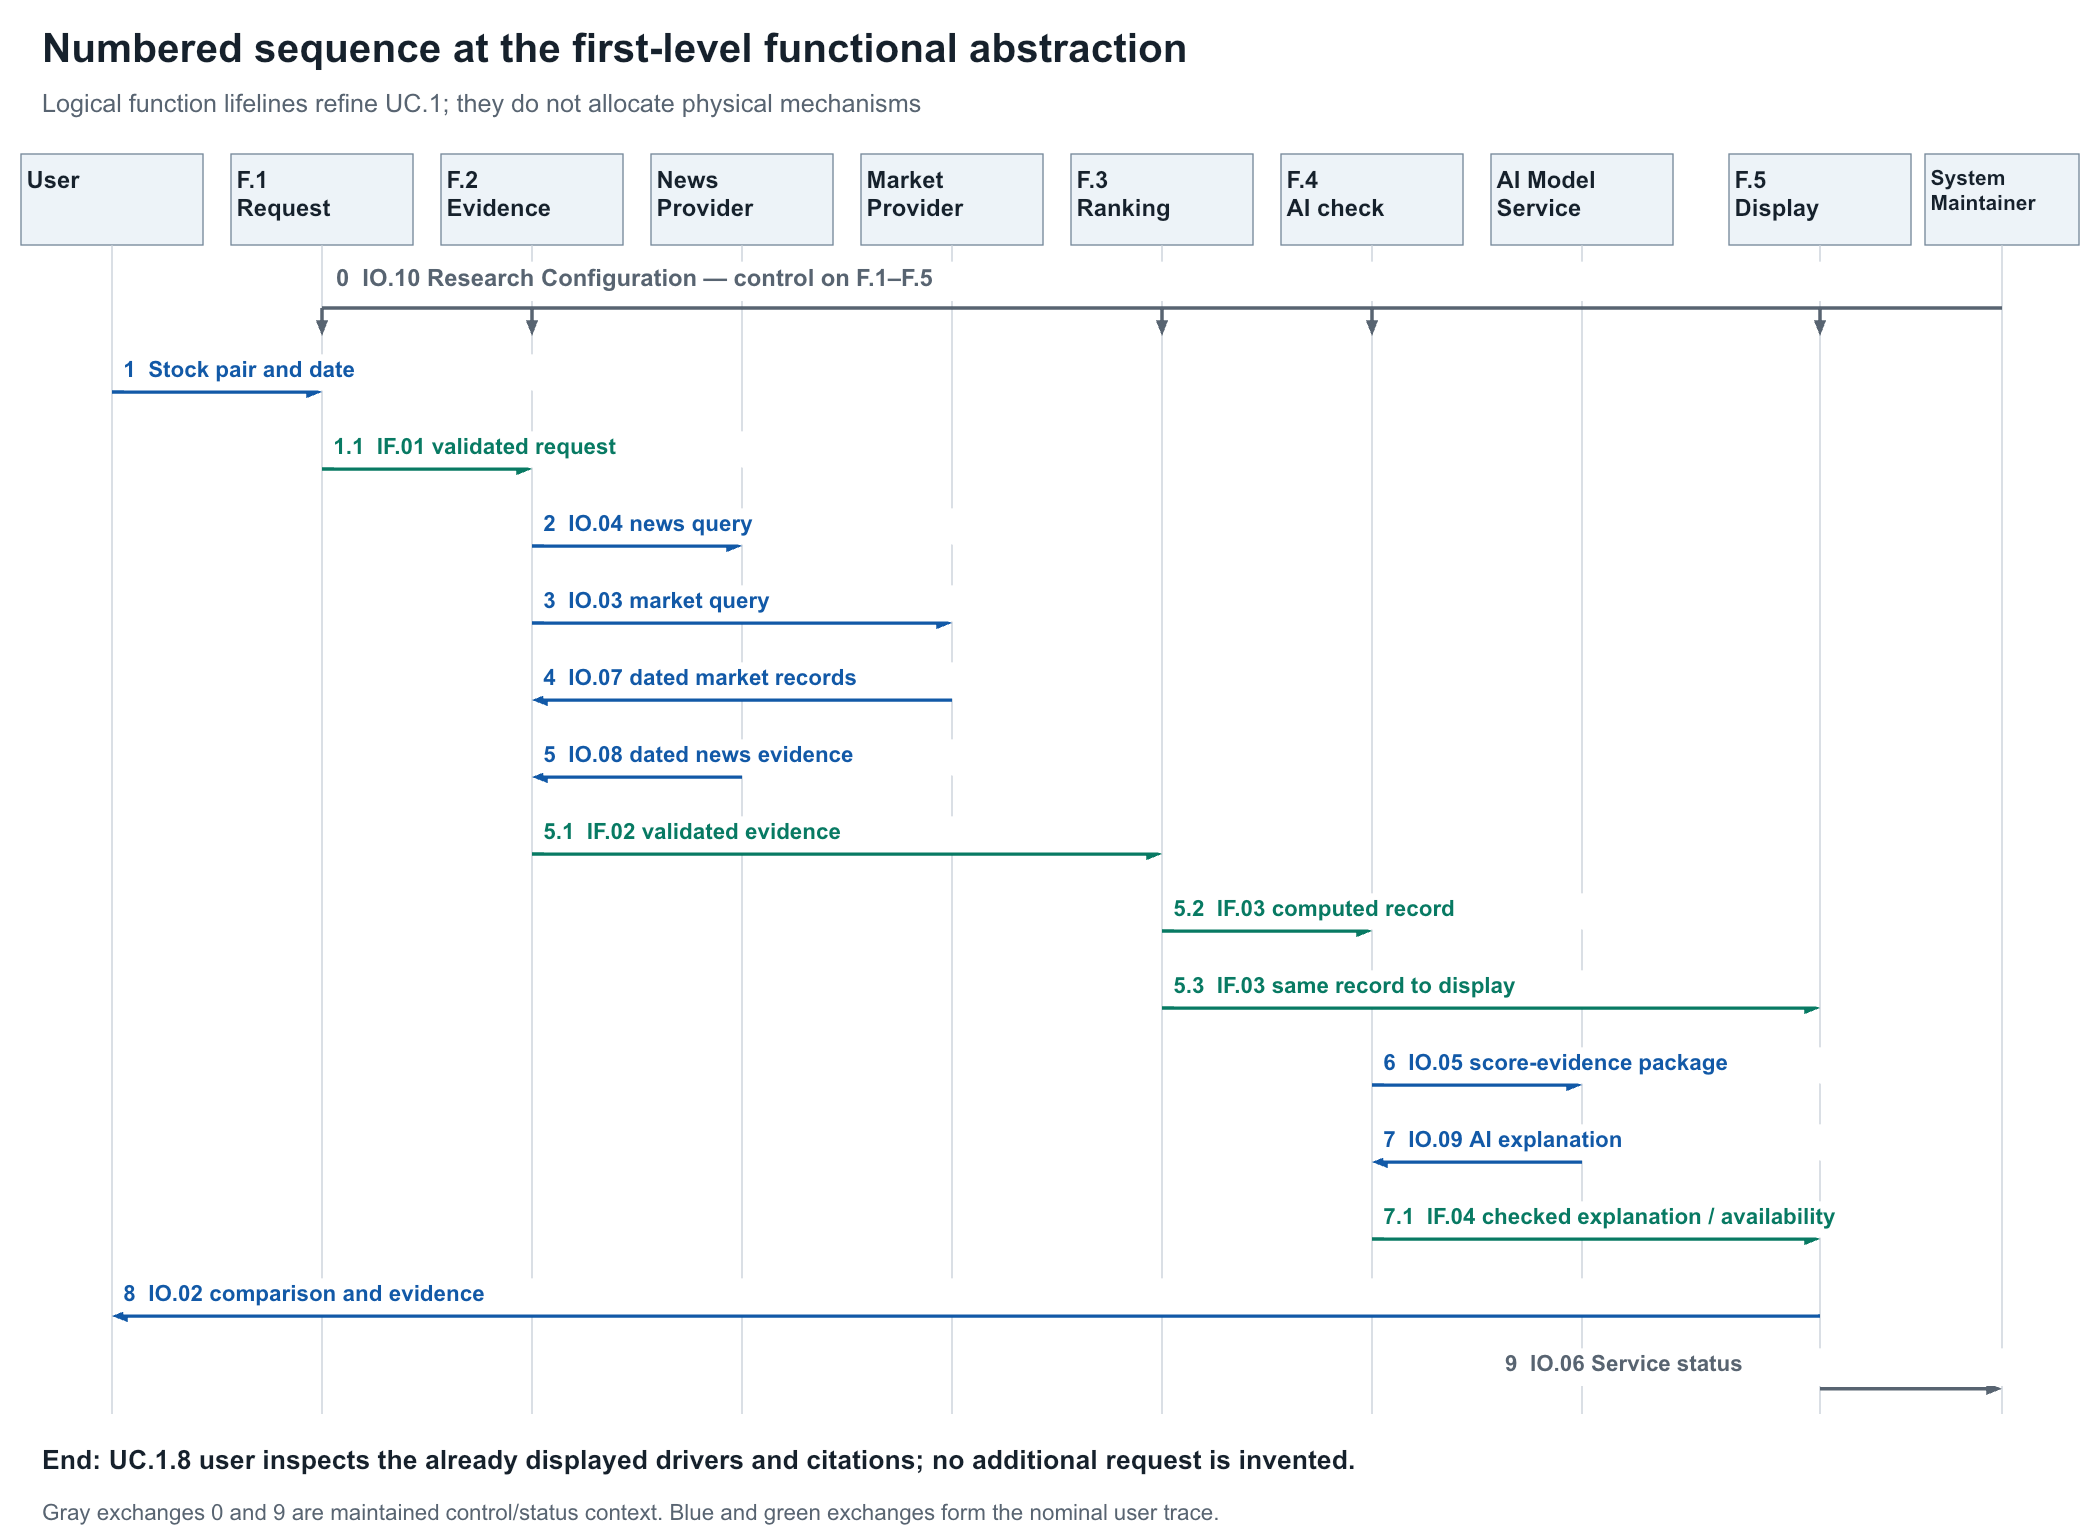
\includegraphics[width=\linewidth,height=.78\textheight,keepaspectratio]{sequence-refined.png}
\caption{Numbered functional refinement of UC.1, including all first-level internal connections.}\label{fig:refined}\end{figure}
\clearpage
\begin{figure}[H]\centering
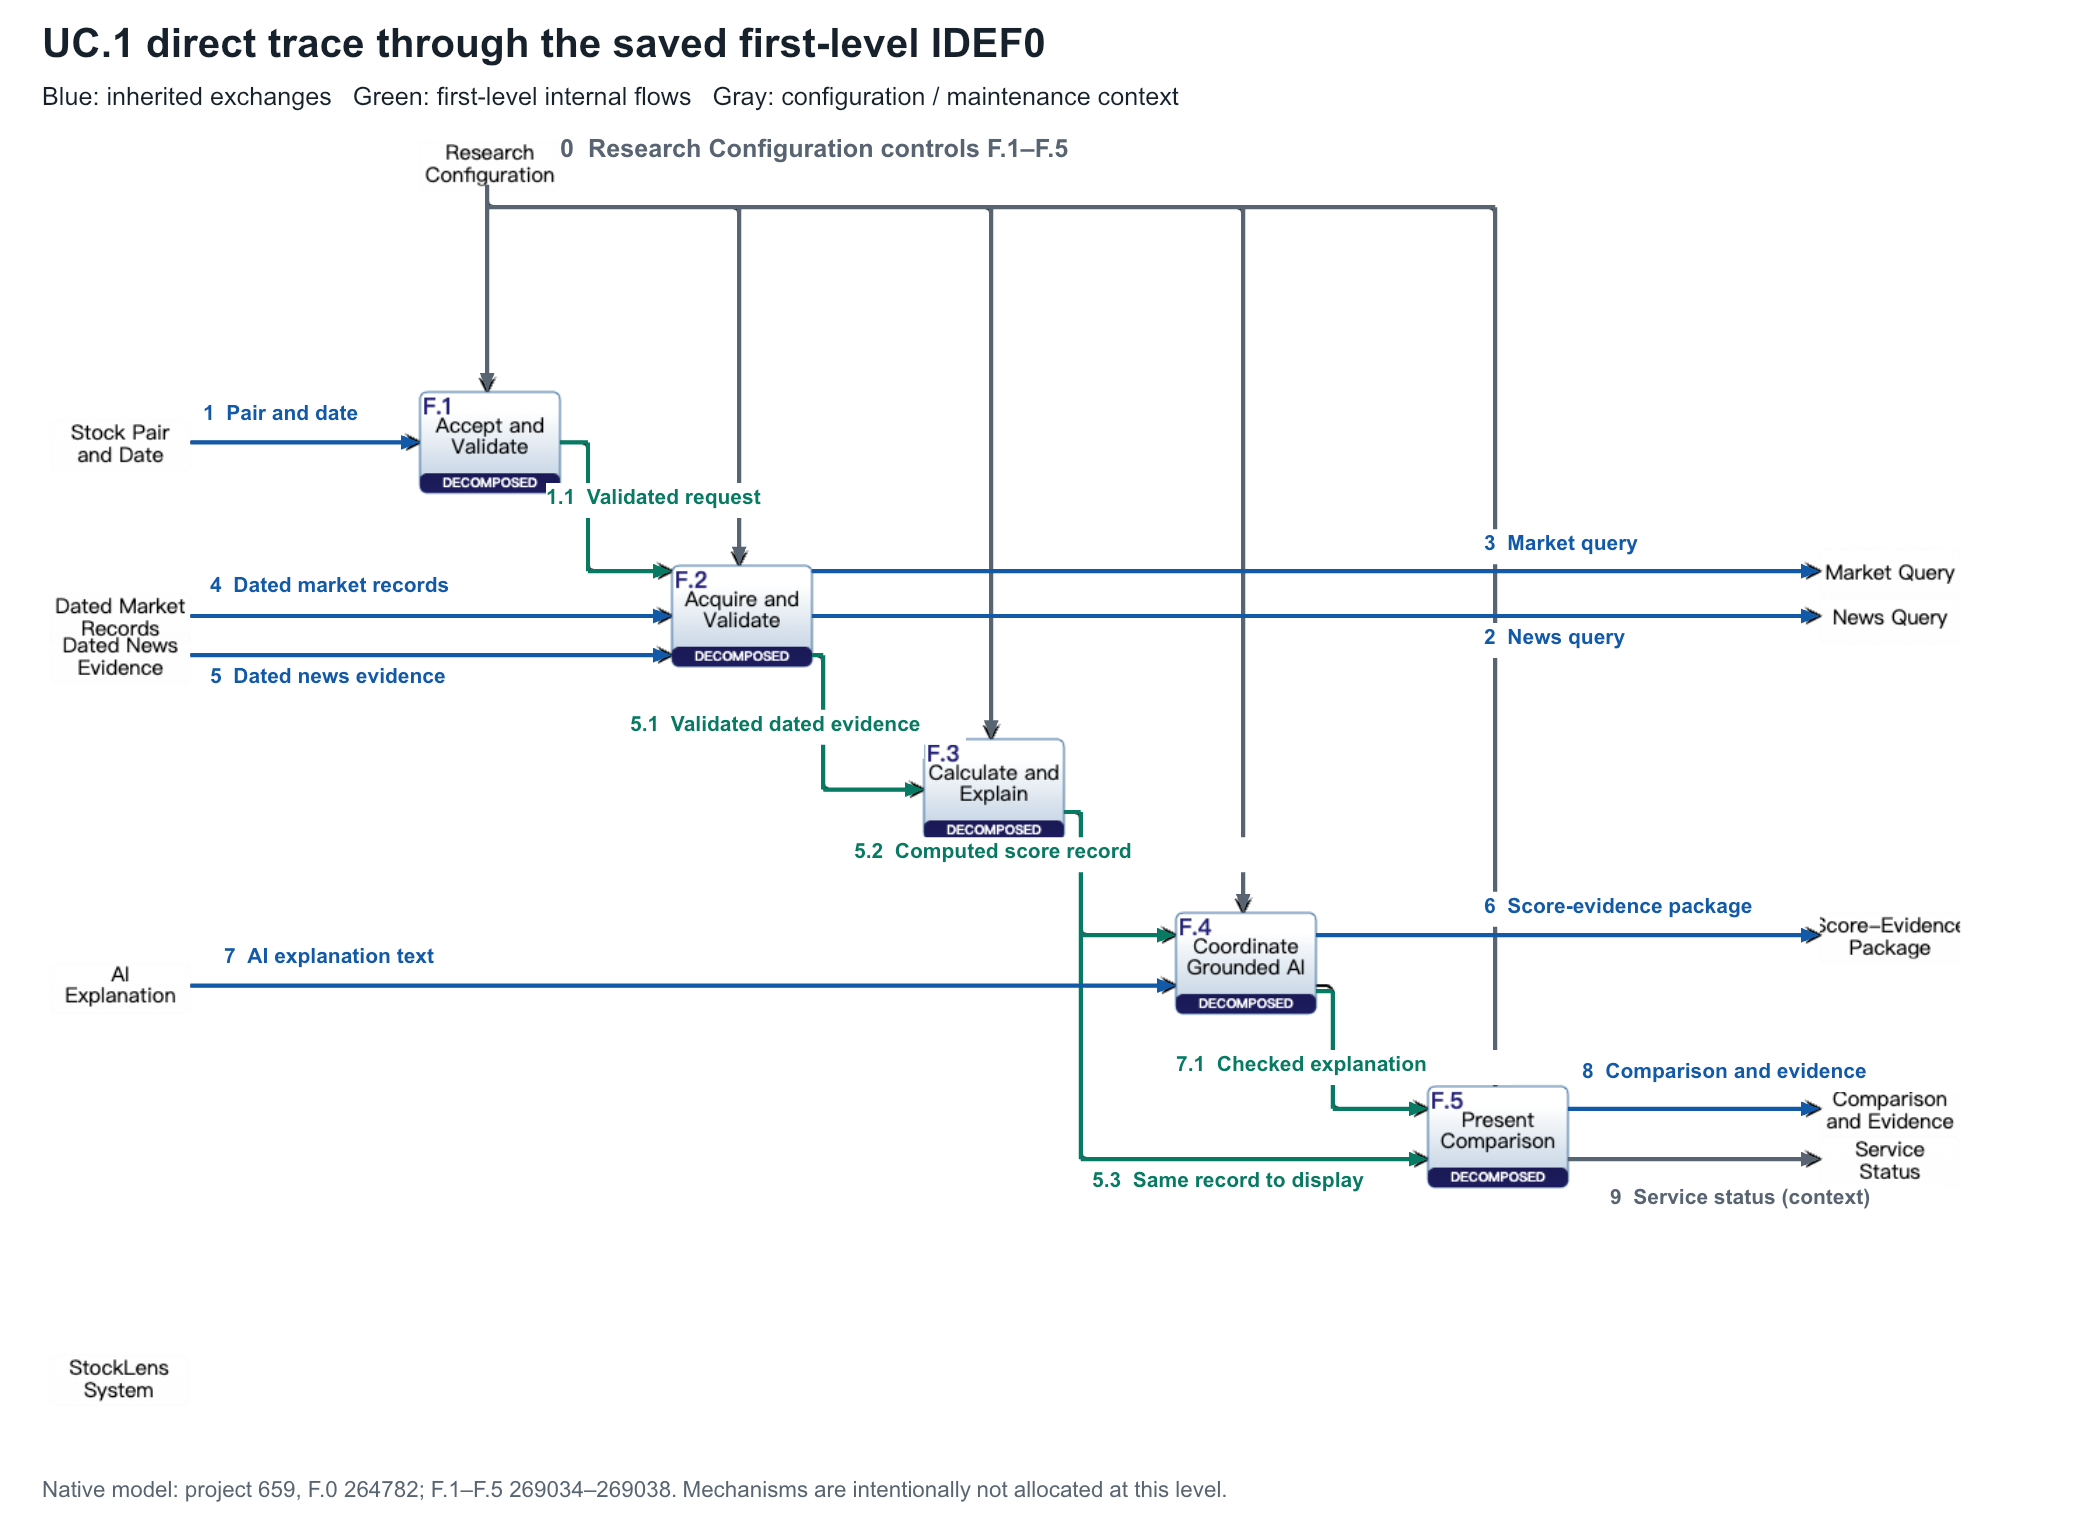
\includegraphics[width=\linewidth,height=.78\textheight,keepaspectratio]{idef0-trace.png}
\caption{Editable PowerPoint annotation over the native first-level IDEF0. Numbers correspond to Figure~\ref{fig:refined}; 0 and 9 retain context outside the nominal user exchange.}\label{fig:trace}\end{figure}
\end{landscape}
{\small
\begin{longtable}{@{}>{\raggedright\arraybackslash}p{0.06\linewidth}>{\raggedright\arraybackslash}p{0.09\linewidth}>{\raggedright\arraybackslash}p{0.28\linewidth}>{\raggedright\arraybackslash}p{0.51\linewidth}@{}}
\caption{Complete trace ledger for the numbered figures.}\\
\toprule Step & Flow & Direction & Action mapping / continuity check\\\midrule\endfirsthead
\toprule Step & Flow & Direction & Action mapping / continuity check\\\midrule\endhead
0 & IO.10 & Maintainer $\rightarrow$ F.1--F.5 & Configuration precondition; baseline controls are carried down.\\[5pt]
1 & IO.01 & User $\rightarrow$ F.1 & UC.1.1--1.2; Comparison Query/API Request Payload refine the user exchange.\\[5pt]
1.1 & IF.01 & F.1 $\rightarrow$ F.2 & Validate request before either provider query.\\[5pt]
2 & IO.04 & F.2 $\rightarrow$ News Provider & UC.1.3.1; dedicated News Fetch Command.\\[5pt]
3 & IO.03 & F.2 $\rightarrow$ Market Provider & UC.1.3.2; dedicated Market Data Fetch Command.\\[5pt]
4 & IO.07 & Market Provider $\rightarrow$ F.2 & UC.1.4.1; retain observation dates.\\[5pt]
5 & IO.08 & News Provider $\rightarrow$ F.2 & UC.1.4.2; retain source and publication dates.\\[5pt]
5.1 & IF.02 & F.2 $\rightarrow$ F.3 & Validated records and request association precede calculation.\\[5pt]
5.2 & IF.03 & F.3 $\rightarrow$ F.4 & UC.1.5 refinement: authoritative computed evidence for AI coordination.\\[5pt]
5.3 & IF.03 & F.3 $\rightarrow$ F.5 & Same computed record supplied directly to display.\\[5pt]
6 & IO.05 & F.4 $\rightarrow$ AI Model Service & UC.1.5/1.6 boundary handoff; approved score-evidence package.\\[5pt]
7 & IO.09 & AI Model Service $\rightarrow$ F.4 & UC.1.6; explanatory return, not a new ranking.\\[5pt]
7.1 & IF.04 & F.4 $\rightarrow$ F.5 & Check narrative against authoritative values; preserve unavailable state.\\[5pt]
8 & IO.02 & F.5 $\rightarrow$ User & UC.1.7 display delivery; UC.1.8 terminal inspection follows.\\[5pt]
9 & IO.06 & F.5 $\rightarrow$ Maintainer & Supplemental inherited operational status, outside nominal UC.1.\\[5pt]
\bottomrule\end{longtable}
}

\subsection{Findings, Corrections and Reconciliation}
The initial screenshot review raised four concerns. Entity-level inspection refined their interpretation and determined the necessary corrections. Table~\ref{tab:findings} separates a genuine structural gap from presentation ambiguities; no earlier observation is retained as a confirmed defect without checking the underlying relationships.
{\small
\begin{longtable}{@{}>{\raggedright\arraybackslash}p{0.1\linewidth}>{\raggedright\arraybackslash}p{0.29\linewidth}>{\raggedright\arraybackslash}p{0.55\linewidth}@{}}
\caption{Review findings and the recorded model corrections.}\label{tab:findings}\\
\toprule Finding & Initial concern & Entity-based resolution\\\midrule\endfirsthead
\toprule Finding & Initial concern & Entity-based resolution\\\midrule\endhead
TR-01 & UC.1.8 was not visible as a sequence arrow. & Entity 185142 already consumed the final display and was performed by the Research User. Its terminal-inspection description and the sequence endpoint note now explain why no extra message is invented.\\[5pt]
TR-02 & A shared Data Fetch Command obscured two provider requests. & Inspection confirmed that both returns had the shared command as input; they were not truly unrequested returns. Dedicated news and market actions/commands now make both exchanges explicit and uniquely numbered.\\[5pt]
TR-03 & The ranking label on an arrow toward AI could imply external calculation. & Entity 186307 was already performed by StockLens. Its name and description now distinguish deterministic local calculation from the outgoing evidence handoff. IF.03 also supplies scores directly to F.5.\\[5pt]
TR-04 & The F.0 decomposition had no first-level functions or internal trace. & Five functions, four internal I/O entities with five directed links, ten lower-level functions, carried-down ICOMs and sixteen requirement allocations are saved. Child interface allocations eliminate newly introduced tunnels.\\[5pt]
\bottomrule\end{longtable}
}

\subsection{Pencil-Test Result and Assessment Limits}
The nominal path is continuous: pair/date $\rightarrow$ F.1 $\rightarrow$ IF.01 $\rightarrow$ F.2; each provider query has its corresponding return; IF.02 enters F.3; IF.03 reaches both F.4 and F.5; F.4 sends the external package and checks the return; IF.04 reaches F.5; the comparison reaches the Research User. Both IF.03 branches are explicit and their destinations are named. No result is attributed to an unrelated function without an internal flow.

The structural review checked five first-level children, two lower-level children per branch, receive/generate inheritance at every branch, absence of first-level mechanism allocation, and coverage of all sixteen existing system requirements. All 22 original structural checks passed against the saved entity records. The submission audit extends these to 64 checks, including direct lower-level/use-case/flow requirement links, six context mechanisms, all inherited ICOMs and exact first-level internal endpoints; all 64 passed. The four first-level internal I/O entities have one generating first-level function each; IF.03 has two receiving functions and the other three have one each. The resulting N-squared cells agree with the IDEF0 and trace ledger.

These checks establish the nominal model's structural continuity, not successful execution of every external-service or human task. Failure handling remains governed by the final requirements baseline: invalid core data yields no ranking, absent qualifying news permits an explicitly calculation-only result, and AI timeout/validation failure preserves valid calculations while marking explanation unavailable. Real-service performance, source permission/support and human comprehension need their own retained evidence.

\section{System Functional Requirements and Traceability}
\subsection{Requirement Form and Measurement Baseline}
The existing sixteen system requirements comprise five accepted exchanges, five provided exchanges, five logical interfaces and one top-level functional requirement. Their original shall statements and identifiers are retained. Functional decomposition supplies more specific satisfaction allocations; it does not create sixteen new stakeholder needs or silently replace the original requirements. Each summary record below includes the upstream source, responsible first-level function, engineering rationale, MOP and verification criterion.

MOP-01 measures common-basis conforming comparisons over assessed comparisons; MOP-02 counts incorrect drivers/values or contradictions of the authoritative breakdown; MOP-03 measures supported, inspectable, correctly dated claims over displayed claims; MOP-04 measures approved-schema-conforming analysis payloads over captured payloads; MOP-05 measures contract-conforming exchanges over assessed exchanges; MOP-06 measures correctly applied configuration/status cases over assessed maintenance cases. The targets are all applicable cases conforming and zero relevant discrepancies in a nonempty recorded set. An empty set is Not Assessed. The $10^{-6}$ score tolerance and other fixed scoring rules remain those of the supplied baseline\cite{baseline}.

\subsection{Requirement Summary}
{\footnotesize
\begin{longtable}{@{}>{\raggedright\arraybackslash}p{0.14\linewidth}>{\raggedright\arraybackslash}p{0.28\linewidth}>{\raggedright\arraybackslash}p{0.27\linewidth}>{\raggedright\arraybackslash}p{0.25\linewidth}@{}}
\caption{Sixteen system requirements: retained obligations, first-level responsibility, rationale and verification criteria.}\\
\toprule Requirement & Retained shall statement / description & Traceability and rationale & MOP and verification criterion\\\midrule\endfirsthead
\toprule Requirement & Retained shall statement / description & Traceability and rationale & MOP and verification criterion\\\midrule\endhead
1.1.1 / 264904\newline Accept Stock Pair and Date & The StockLens System shall accept Stock Pair and Date from the Research User. & \textbf{Upstream:} SR-01  Comparable stock results\newline\textbf{Allocation:} F.1\newline\textbf{Rationale:} The intended pair/date must survive request validation. & \textbf{MOP:} 01,05\newline V-111: accepted symbols and date exactly match a valid submitted request; invalid/duplicate/out-of-universe symbols or invalid dates produce no ranking.\\[5pt]
1.1.2 / 264903\newline Accept Dated Market Records & The StockLens System shall accept Dated Market Records from the Market Data Provider. & \textbf{Upstream:} SR-01  Comparable stock results; SR-03  Dated supporting evidence\newline\textbf{Allocation:} F.2\newline\textbf{Rationale:} Comparable scoring needs attributable market observations. & \textbf{MOP:} 01,05\newline V-112: preserve request association, symbol coverage, adjusted-price observations and dates; reject insufficient aligned coverage.\\[5pt]
1.1.3 / 264902\newline Accept Dated News Evidence & The StockLens System shall accept Dated News Evidence from the News Provider. & \textbf{Upstream:} SR-03  Dated supporting evidence\newline\textbf{Allocation:} F.2\newline\textbf{Rationale:} News must remain attributable to inspected items. & \textbf{MOP:} 03,05\newline V-113: preserve source identifiers and publication dates; inspect that each associated claim is supported by the referenced item.\\[5pt]
1.1.4 / 264901\newline Accept AI Explanation Text & The StockLens System shall accept AI Explanation Text from the AI Model Service. & \textbf{Upstream:} SR-02  Ranking explanation; SR-03  Dated supporting evidence\newline\textbf{Allocation:} F.4\newline\textbf{Rationale:} AI text explains authoritative scores rather than replacing them. & \textbf{MOP:} 02,03,05\newline V-114: driver values and source references agree with the supplied record; reject inconsistent text without changing numerical ranking.\\[5pt]
1.1.5 / 264900\newline Accept Research Configuration & The StockLens System shall accept Research Configuration from the System Maintainer. & \textbf{Upstream:} SR-01  Comparable stock results; SR-07  Provider conditions; SR-08  Approved AI request schema\newline\textbf{Allocation:} F.1; control on F.1--F.5\newline\textbf{Rationale:} One version governs the entire comparison. & \textbf{MOP:} 01,04,06\newline V-115: the accepted version is the one used for eligibility, common calculation basis, permitted analysis content and status reporting.\\[5pt]
1.2.1 / 264899\newline Provide Comparison and Evidence & The StockLens System shall provide Comparison and Evidence to the Research User. & \textbf{Upstream:} SR-01  Comparable stock results; SR-02  Ranking explanation; SR-03  Dated supporting evidence\newline\textbf{Allocation:} F.5\newline\textbf{Rationale:} The result must combine values, drivers, dates and support coherently. & \textbf{MOP:} 01,02,03\newline V-121: displayed values match independent calculations; drivers and claim/source/date associations are correct.\\[5pt]
1.2.2 / 264898\newline Provide Market Query & The StockLens System shall provide Market Query to the Market Data Provider. & \textbf{Upstream:} SR-01  Comparable stock results; SR-07  Provider conditions\newline\textbf{Allocation:} F.2\newline\textbf{Rationale:} The market query must request the authorized observations. & \textbf{MOP:} 05\newline V-122: capture the query and verify selected provider, intended symbols, common window and permitted access.\\[5pt]
1.2.3 / 264897\newline Provide News Query & The StockLens System shall provide News Query to the News Provider. & \textbf{Upstream:} SR-03  Dated supporting evidence; SR-07  Provider conditions\newline\textbf{Allocation:} F.2\newline\textbf{Rationale:} Company/date bounds determine relevant news evidence. & \textbf{MOP:} 03,05\newline V-123: capture provider destination and company/date filters; keep returned items associated with the intended query.\\[5pt]
1.2.4 / 264896\newline Provide Score-Evidence Package & The StockLens System shall provide Score-Evidence Package to the AI Model Service. & \textbf{Upstream:} SR-02  Ranking explanation; SR-03  Dated supporting evidence; SR-08  Approved AI request schema\newline\textbf{Allocation:} F.4\newline\textbf{Rationale:} AI needs checked calculation and source context. & \textbf{MOP:} 02,03,04\newline V-124: request matches computed values and permitted schema; credentials and unnecessary personal data are excluded; invalid content is not transmitted.\\[5pt]
1.2.5 / 264895\newline Provide Service Status & The StockLens System shall provide Service Status to the System Maintainer. & \textbf{Upstream:} SR-06  Operation and transition guide\newline\textbf{Allocation:} F.5\newline\textbf{Rationale:} The maintainer needs the observed workflow state. & \textbf{MOP:} 05,06\newline V-125: status corresponds to the operation and applied configuration using the recorded five-state dictionary.\\[5pt]
1.3.1 / 264894\newline User Research Interface & The StockLens System shall interface with the Research User through the User Research Interface. & \textbf{Upstream:} SR-01  Comparable stock results; SR-02  Ranking explanation; SR-03  Dated supporting evidence\newline\textbf{Allocation:} F.1 request; F.5 result\newline\textbf{Rationale:} The same comparison must connect request and display. & \textbf{MOP:} 01,02,03,05\newline V-131: request/result identity and endpoint directions agree; display includes driver/source/date context; fixtures are never relabelled as requested real data.\\[5pt]
1.3.2 / 264893\newline Market Data Interface & The StockLens System shall interface with the Market Data Provider through the Market Data Interface. & \textbf{Upstream:} SR-01  Comparable stock results; SR-07  Provider conditions\newline\textbf{Allocation:} F.2\newline\textbf{Rationale:} Market queries and responses form one logical provider interface. & \textbf{MOP:} 05\newline V-132: paired endpoints, symbols, units and observation periods agree with the frozen provider contract.\\[5pt]
1.3.3 / 264892\newline News Interface & The StockLens System shall interface with the News Provider through the News Interface. & \textbf{Upstream:} SR-03  Dated supporting evidence; SR-07  Provider conditions\newline\textbf{Allocation:} F.2\newline\textbf{Rationale:} News exchanges must preserve provenance and permitted use. & \textbf{MOP:} 03,05\newline V-133: query/response association and source/date fields are correct; inspect retention/display against dated provider conditions.\\[5pt]
1.3.4 / 264891\newline AI Analysis Interface & The StockLens System shall interface with the AI Model Service through the AI Analysis Interface. & \textbf{Upstream:} SR-02  Ranking explanation; SR-03  Dated supporting evidence; SR-08  Approved AI request schema\newline\textbf{Allocation:} F.4\newline\textbf{Rationale:} Explanatory exchange must preserve ranking ownership. & \textbf{MOP:} 02,03,04,05\newline V-134: the outgoing checked package and returned text share comparison identity; invalid schema or inconsistent claims are rejected.\\[5pt]
1.3.5 / 264890\newline Maintenance Interface & The StockLens System shall interface with the System Maintainer through the Maintenance Interface. & \textbf{Upstream:} SR-06  Operation and transition guide\newline\textbf{Allocation:} F.5 status; configuration control\newline\textbf{Rationale:} Configuration and status form the maintenance loop. & \textbf{MOP:} 05,06\newline V-135: identify the maintainer, accepted/applied configuration version and returned observed status; independent handover requires its own demonstration.\\[5pt]
1.4.1 / 264940\newline Provide Stock Comparisons & The StockLens System shall provide evidence-linked comparisons of two eligible stocks using a common analysis date and a documented indicator and scoring configuration. & \textbf{Upstream:} SR-01  Comparable stock results; SR-02  Ranking explanation; SR-03  Dated supporting evidence\newline\textbf{Allocation:} F.3 with F.1--F.5 integration\newline\textbf{Rationale:} A research request needs comparable calculations, explanations and dated evidence. & \textbf{MOP:} 01,02,03\newline V-141: compare a complete nonempty set against independent score/driver calculations and checked sources; correct degradation preserves scores and exposes unavailable support.\\[5pt]
\bottomrule\end{longtable}
}

\subsection{Requirements Management and Evidence Status}
Native satisfaction relations now allocate the sixteen requirements across F.1--F.5; F.0 retains overall responsibility. F.1 carries the request/configuration and user-interface obligations, F.2 carries acquisition and provider-interface obligations, F.3 carries the top-level comparison calculation, F.4 carries the AI package/return/interface obligations, and F.5 carries comparison delivery, service status and maintenance-interface obligations. The user interface spans both request and result directions even where a single native allocation records its principal owner.

The requirement diagram retains the native upstream and verification relationships. A satisfaction or verified-by link is not a passed test. The supplied final requirements report records prior controlled results and full-plan limitations; this revision does not relabel those historical runs as new external-service or stakeholder observations. No user-study participants, live provider selection, real AI behavior or external-service latency measurements are claimed here.
\begin{figure}[H]\centering
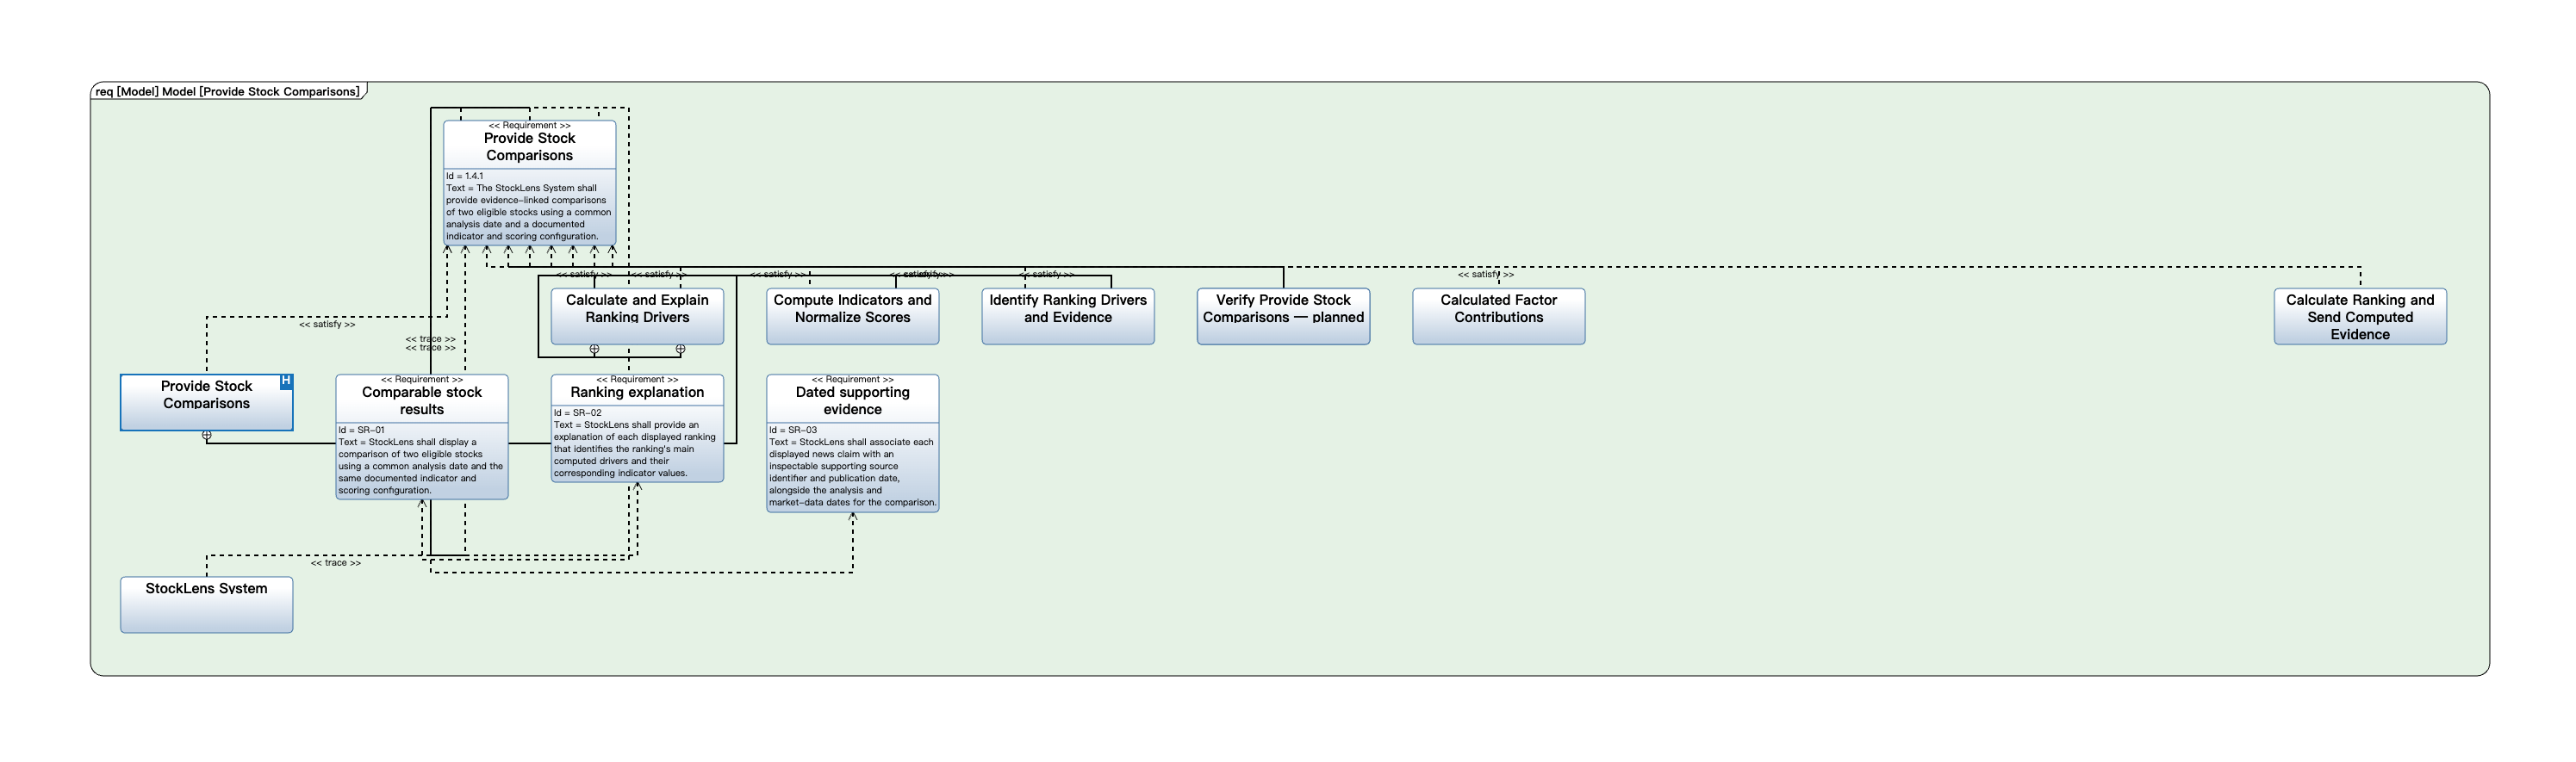
\includegraphics[width=\linewidth,height=.78\textheight,keepaspectratio]{requirements-traceability.png}
\caption{Native requirement traceability view rooted at 1.4.1 (264940), including its current satisfaction and upstream relationships.}\label{fig:reqtrace}\end{figure}

\section{Actual Operations and Reproducible Evidence}
The model work was executed in Innoslate, not only drafted in this report. Saved operations include five first-level function entities, ten lower-level function entities, four first-level internal I/O entities, five lower-level connecting flows, carried-down input/control/output relations, sixteen first-level requirement allocations, the distinct news-query action and command, and clarification of ranking ownership and terminal inspection. Existing context exchange and system-requirement IDs were reused.

The evidence package contains native PNG exports, the editable two-slide PowerPoint trace, UI-read entity/relationship records, the use-case baseline record and the 22-check consistency result. Those records can be compared with the live model by stable entity ID. A model change after export requires rechecking and re-exporting the affected figures; successful LaTeX compilation alone is not a model-consistency check.

\subsection{Native Intelligence Review and Disposition}
Innoslate Intelligence was rerun on project 659 after the corrections. It analyzed 266 entities, including 76 Actions and 30 Input/Outputs. Fourteen lower-level/use-case Actions and eighteen derived I/O entities received direct requirement links. The final native I/O Analysis passes all six applicable heuristics (100\%). The machine-readable model audit independently passes 64 checks; it does not use the project's global heuristic percentage as an acceptance score.

\begin{longtable}{@{}>{\raggedright\arraybackslash}p{.28\linewidth}>{\raggedright\arraybackslash}p{.66\linewidth}@{}}\toprule
Finding class & Disposition for this assignment\\\midrule\endhead
Missing requirement links on current lower-level/use-case Actions and derived flows & Corrected in the live model. Ten lower-level functions, four use-case actions and eighteen derived I/O records now have direct links to the corresponding retained requirements.\\[4pt]
No performing Asset on first-level/lower-level functions & Accepted staged exception under Lab Manual 7.2.2. The six functions actually shown on the context IDEF0 each retain exactly one mechanism. No premature physical architecture is invented.\\[4pt]
Multiple I/O records satisfying one requirement & Accepted refinement: the same boundary obligation is realized by the carried-down interface and its lower-level request/evidence handoffs. The trace ledger and contract identify the distinct flows; this is not an unresolved duplicate flow.\\[4pt]
Ambiguous-word heuristics on current names/descriptions & Reviewed in context. ``Common'' means the same recorded analysis date; ``Present'' is the required verb in F.5; ``both'' denotes exactly the two selected symbols. Full definitions and contract fields remove referential ambiguity.\\[4pt]
Old airport requirements, unnamed exploratory entities and legacy subsystem findings & Retained as historical/out-of-scope findings, not deleted to inflate a score. Their text and the final raw Intelligence output are retained in the evidence package. They are not members of the selected StockLens F.0 hierarchy or the sixteen-row requirement baseline.\\[4pt]
Physical conduit completeness at AI/UI/user assets & Deferred physical-interface follow-up. Functional I/O continuity is checked at the selected context and first level; conduit/subsystem allocation follows the physical-architecture lesson and is not falsely closed by this functional audit.\\[4pt]
Unallocated logical containers, human-inspection and planned verification actions & Reviewed as containers, included user behavior or verification plans rather than unimplemented first-level calculations. Their links are not represented as passed human or product tests.\\\bottomrule\end{longtable}

\begin{figure}[H]\centering
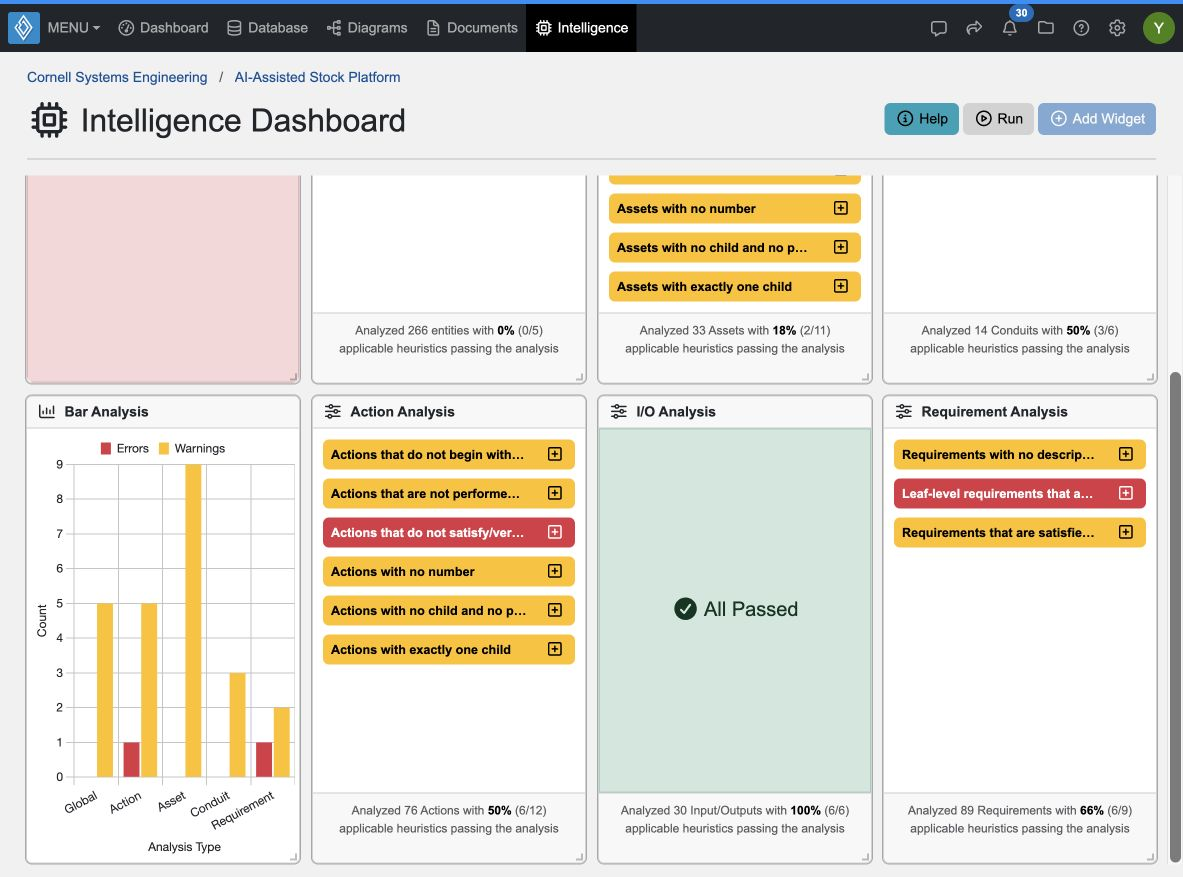
\includegraphics[width=\linewidth,height=.65\textheight,keepaspectratio]{intelligence-verified.png}
\caption{Native Intelligence evidence retained after correction. Global legacy findings remain visible and have scoped dispositions.}\label{fig:intelligence}\end{figure}

\subsection{Chapter 6.4: Product Entry-Point Audit}
The actual product baseline was located in the retained StockLen repository at commit a1f7067, the source of the prior requirements report's controlled verification. Work was performed in an isolated copy. The older SYSEN5151 walking skeleton was not mistaken for that later baseline. The delivered product source records the complete audit in \texttt{docs/route-table.md}.

Ten HTTP routes were found before the audit. The automatically exposed Swagger, ReDoc and public OpenAPI routes had no modeled user task and were disabled. Seven explicit routes remain: two legacy fixture routes (\texttt{GET /} and \texttt{POST /compare}) and five controlled research routes (page, comparison, status, configuration and inspectable source). The current comparison route traces to UC.1 and F.1--F.5; status/configuration trace to the already modeled maintainer context at steps 0 and 9; source inspection supports UC.1.8 and the included source-inspection behavior. A runtime test fixes the final route set, so a hidden documentation endpoint cannot silently reappear.

The audit also enumerates browser events and launch/build/verification commands. The inherited historical sandbox allowed a different sentiment-weighted scoring method, more than two selected stocks and subsequent-return inspection. Its four interactive control groups and dead scripts were removed from the delivered product copy. The retained fixed-fixture mirror is clearly labeled and cannot relabel demonstration values as a real requested result. Lifecycle and verification commands are traced to their support purpose, not counted as extra research use cases. Human inspection remains a user action over displayed evidence; it is not assigned a fabricated calculation endpoint. The entry-point mapping is retained for review.

\subsection{Chapter 7.4: Internal Contract Before Refactoring}
The authority chain is the saved model's flow list, then \texttt{contracts/api-v1.yaml}, then generated server signatures/client methods, then the implementation. The OpenAPI 3.1 contract is written in JSON-compatible YAML and defines all four internal flows and five directed connections. It specifies operation request/response schemas, types, price/ratio/score units, configuration identity, date/source association and failure behavior. The logical operation paths document in-process boundaries; they are not additional public endpoints.

\begin{tabularx}{\linewidth}{@{}p{.15\linewidth}p{.28\linewidth}X@{}}\toprule
Flow & Operation / destination & Contracted exchange\\\midrule
IF.01 & F.2 acquire\_evidence & ValidatedRequest to DatedEvidence; reject extra fields, wrong configuration version or ineligible request.\\
IF.02 & F.3 calculate\_ranking & DatedEvidence to ComputedRecord; retain the full ten-stock normalization universe and reject missing/nonpositive/nonfinite observations.\\
IF.03 & F.4 check\_explanation; F.5 presentation join & One ComputedRecord is copied to both destinations. AI receives only the checked score/evidence package; no narrative may replace numerical scores.\\
IF.04 & F.5 present\_comparison & CheckedExplanation includes comparison identity, availability and checked text or null; mismatched identity is rejected.\\\bottomrule\end{tabularx}

The generated client validates every internal request and response. FunctionalServer implements F.1--F.5, and ResearchRuntime follows those boundaries once per comparison. The former duplicate calculation around AI coordination is removed; the F.0 public facade is retained for compatibility. Configuration remains an immutable injected control snapshot, with its version checked at every handoff. ADR-0004 records this divergence and names F.0, F.1--F.5, IF.01--IF.04 and the affected requirement entities. The contract and implementation are versioned in the delivered local repository and its reproducible source archive. The designated GitHub report folder includes that product evidence archive without silently replacing the separate historical application baseline.

\subsection{Executed Verification and Reproduction}
All 34 Python unit/integration tests passed: 26 retained tests, including the sixteen requirement-linked controlled cases and independent Decimal/direct-counting arithmetic, plus eight new contract/route tests. The new tests check schema rejection on both request and response, configuration mismatch, unrelated explanation identity, immutable score fan-out, the five-function execution order, generated-contract hash agreement and the final public route set. Three additional JavaScript checks passed for browser-fixture parity, preservation of fixture/request identity and removal of orphan website controls with a clean static-site build. The two retired sandbox tests were replaced because their feature was removed; scoring conformance remains covered by the independent Python oracle. A separate deliberately corrupted ranking helper is rejected by the independent oracle; the tests are not weakened to match the implementation.

Actual loopback HTTP checks passed for request preservation, invalid symbols/date rejection, status/configuration behavior and resolvable synthetic source links. Twenty serial offline comparison requests were executed. Their descriptive nearest-rank P95 was 0.003376 seconds; this is local synthetic API timing, not a browser-complete or real-service latency claim. The actual browser was also exercised: a valid comparison displayed two-decimal scores, both computed drivers and source/publication dates; an unknown symbol cleared the old result and displayed a failure. The screenshot below is from that run. No external provider or AI request was made.

\begin{figure}[H]\centering
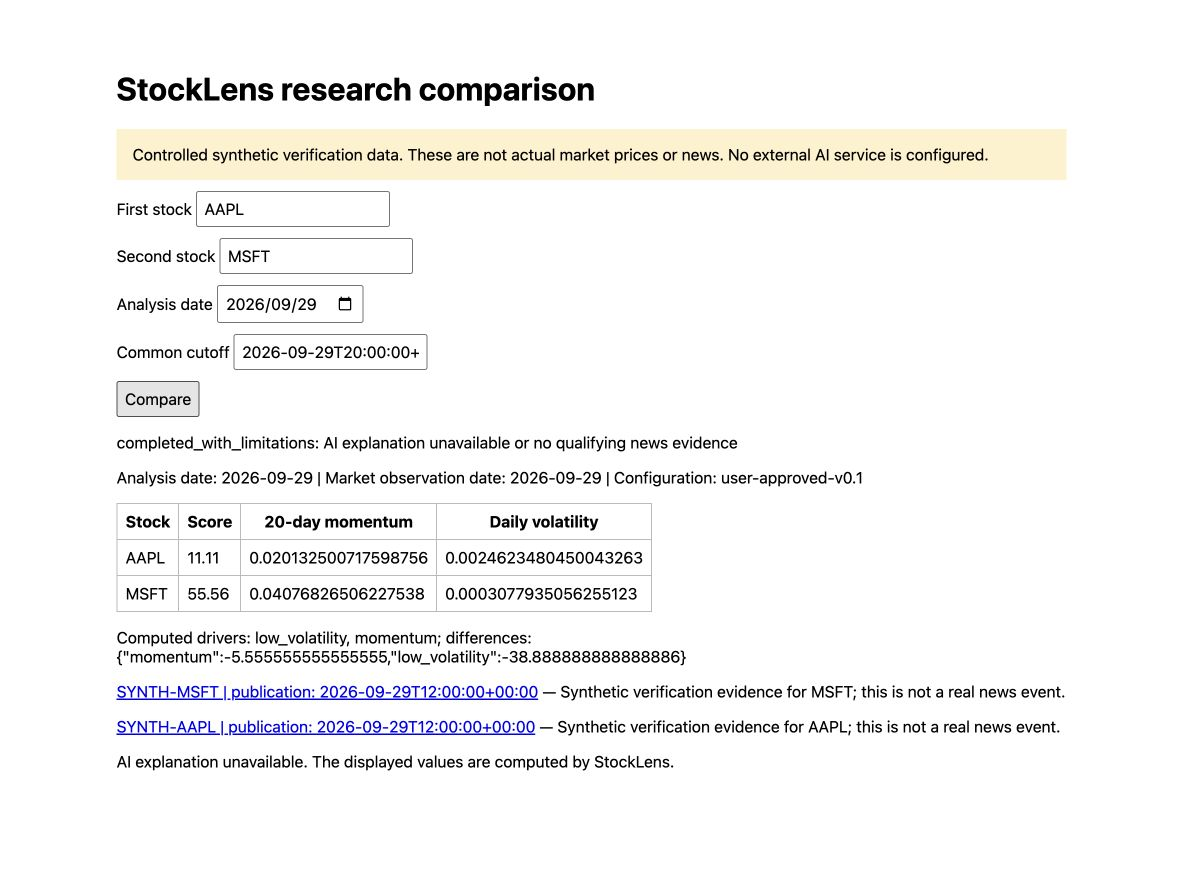
\includegraphics[width=\linewidth,height=.64\textheight,keepaspectratio]{browser-verified.png}
\caption{Actual browser execution of the refactored controlled product. Synthetic provenance and unavailable external AI are explicitly displayed.}\label{fig:browser}\end{figure}

To reproduce, extract \texttt{StockLens\_Chapter6\_7\_Product.zip}; install \texttt{requirements-ch4-lock.txt} into a virtual environment; regenerate with \texttt{python scripts/generate\_internal\_stubs.py}; run \texttt{python -m unittest discover -s tests -v} and \texttt{python scripts/check\_ch4\_http.py}. Start \texttt{python -m walking\_skeleton} and open \texttt{http://127.0.0.1:8765/research}. The product archive includes source, the exact internal contract, generated stubs, ADR, entry-point table and new evidence logs. The report package separately includes native model records, all 64 structural check results and the editable PowerPoint trace.

\subsection{Submission Boundary}
The deliverable is one integrated PDF containing the Chapter 6 tracework and Chapter 7 architecture, with explanatory text, ICOM, three-level hierarchy, readable branch projections, N-squared view, requirement rationale/MOP/verification table and team contributions. One saved first-level IDEF0 is the common baseline for the tracing figures. PowerPoint and machine-readable/source evidence accompany the PDF as supporting artifacts; they do not replace the required Word/PDF submission format.

The supplied requirements report's unperformed real-service tests, independent handover and stakeholder studies remain unperformed; architecture verification criteria do not imply those tests have passed. The native global heuristic findings are disclosed with scoped dispositions rather than misrepresented as a clean global project. Canvas remains unsubmitted; this package prepares the artifacts for submission.

\section{Summary}
The revised model has a three-level functional hierarchy and a first-level IDEF0 with complete inherited ICOM allocation and four named internal exchanges. The N-squared view records five directed internal connections, including the authoritative score-record fan-out. Independent provider queries and clarified message names make the native use-case view easier to reconcile with the functional architecture. The numbered PowerPoint IDEF0 trace and function-level sequence use one common ledger and expose every first-level handoff needed by the selected nominal scenario.

All 64 submission-model checks and all 34 controlled software tests passed. The model, numbered diagrams, machine-readable interface contract and refactored F.1--F.5 implementation agree on the four internal flows and five directed links. Live-provider suitability and stakeholder comprehension remain governed by their separate evidence and acceptance criteria.

\section{Team Contribution Table}
The table separates assigned responsibilities for this submission from previously recorded contribution evidence. The assigned work is not presented as a new independently verified completion record. N/A indicates no completed contribution reported for this assignment.
\par\noindent\begin{tabularx}{\linewidth}{@{}p{.22\linewidth}X@{}}\toprule
Student & Assigned responsibility and recorded contribution\\\midrule
Yihan Zhou & Report integration, model consistency and product verification. Coordinated model and report revisions, contract refactoring and verification.\\
Shuxuan Wang & Functional hierarchy and IDEF0 discussion. Earlier team contribution: non-functional candidates, stakeholder/MOS links and technical risks reused as architecture drivers.\\
Henian Li & Functional requirements, MOPs and verification table. Earlier team contribution: sixteen-row RVTM, verification criteria and evidence review retained as the requirement baseline.\\
Xinyuan Yan & Use-case tracing, N-squared analysis and interface review. Earlier team contribution: functional architecture diagrams, relationships and ICOM consistency review reused as the model baseline.\\
David Limmer & N/A\\
Rosa Szurgot & N/A\\\bottomrule\end{tabularx}\par

\begin{thebibliography}{9}
\bibitem{manual} SYSEN 5151. \textit{Foundations of Systems Engineering Lab Manual}, Version 3.0, September 7, 2026. Sections 6.2.1, 6.3--6.4, 7.2--7.4 and related assessment criteria.
\bibitem{assignment} SYSEN 5151. \href{https://canvas.cornell.edu/courses/92732/assignments/981139}{\textit{Architecture Definition: Function}}, Canvas assignment and 100-point rubric. Due October 25, 2026.
\bibitem{baseline} Group 29. \textit{StockLens System Requirements Definition}, final report supplied by the user, October 18, 2026; authorized baseline v0.1, original system requirements and verification limits.
\bibitem{model} Group 29. \href{https://cloud.innoslate.com/cornell/p/659/diagrams}{\textit{AI-Assisted Stock Platform}}, Innoslate project 659. Model entities and native figures reviewed for this revision.
\end{thebibliography}
\appendix
\section{Rubric Coverage and Evidence Index}
\par\noindent\begin{tabularx}{\linewidth}{@{}p{.31\linewidth}p{.08\linewidth}X@{}}\toprule
Criterion & Points & Evidence in this report\\\midrule
Integrated report & 5 & Purpose, modeling rationale, assumptions, coherent discussion and contribution table.\\
Flow consistency & 40 & Corrected native use case, two numbered trace figures, complete mapping ledger, resolved findings and scoped pencil test.\\
IDEF0 & 25 & Native context/first-level figures, all ten inherited ICOMs, four internal exchanges and boundary discussion.\\
Function hierarchy & 10 & Three-level native overview, five readable branch projections and complete lower-level definitions.\\
Functional requirements & 15 & Sixteen retained shall statements, upstream relationships, descriptions, rationale, MOPs and verification criteria.\\
N-squared & 5 & Native matrix and explicit interpretation of all five internal connections.\\\bottomrule
\end{tabularx}\par
The table records deliverable coverage, not a predicted grade. The package retains model snapshots, 64 model checks, 34 executed controlled tests, HTTP/browser evidence and a contract-first product source archive. Unperformed real-service and human validation are not inferred from report completeness.
\end{document}
